%% bare_jrnl_transmag.tex
%% V1.4b
%% 2015/08/26
%% by Michael Shell
%% see http://www.michaelshell.org/
%% for current contact information.
%%
%% This is a skeleton file demonstrating the use of IEEEtran.cls
%% (requires IEEEtran.cls version 1.8b or later) with an IEEE 
%% Transactions on Magnetics journal paper.
%%
%% Support sites:
%% http://www.michaelshell.org/tex/ieeetran/
%% http://www.ctan.org/pkg/ieeetran
%% and
%% http://www.ieee.org/

%%*************************************************************************
%% Legal Notice:
%% This code is offered as-is without any warranty either expressed or
%% implied; without even the implied warranty of MERCHANTABILITY or
%% FITNESS FOR A PARTICULAR PURPOSE! 
%% User assumes all risk.
%% In no event shall the IEEE or any contributor to this code be liable for
%% any damages or losses, including, but not limited to, incidental,
%% consequential, or any other damages, resulting from the use or misuse
%% of any information contained here.
%%
%% All comments are the opinions of their respective authors and are not
%% necessarily endorsed by the IEEE.
%%
%% This work is distributed under the LaTeX Project Public License (LPPL)
%% ( http://www.latex-project.org/ ) version 1.3, and may be freely used,
%% distributed and modified. A copy of the LPPL, version 1.3, is included
%% in the base LaTeX documentation of all distributions of LaTeX released
%% 2003/12/01 or later.
%% Retain all contribution notices and credits.
%% ** Modified files should be clearly indicated as such, including  **
%% ** renaming them and changing author support contact information. **
%%*************************************************************************


% *** Authors should verify (and, if needed, correct) their LaTeX system  ***
% *** with the testflow diagnostic prior to trusting their LaTeX platform ***
% *** with production work. The IEEE's font choices and paper sizes can   ***
% *** trigger bugs that do not appear when using other class files.       ***                          ***
% The testflow support page is at:
% http://www.michaelshell.org/tex/testflow/



% \documentclass[journal,transmag]{IEEEtran}
\documentclass[12pt, onecolumn, journal]{IEEEtran}
\usepackage[margin=1in]{geometry} % 1-inch margins on all sides
\usepackage{setspace} % Package for line spacing
\usepackage{times} % Use Times New Roman font
\doublespacing % Set double line spacing
%
% If IEEEtran.cls has not been installed into the LaTeX system files,
% manually specify the path to it like:
% \documentclass[journal]{../sty/IEEEtran}





% Some very useful LaTeX packages include:
% (uncomment the ones you want to load)


% *** MISC UTILITY PACKAGES ***
%
%\usepackage{ifpdf}
% Heiko Oberdiek's ifpdf.sty is very useful if you need conditional
% compilation based on whether the output is pdf or dvi.
% usage:
% \ifpdf
%   % pdf code
% \else
%   % dvi code
% \fi
% The latest version of ifpdf.sty can be obtained from:
% http://www.ctan.org/pkg/ifpdf
% Also, note that IEEEtran.cls V1.7 and later provides a builtin
% \ifCLASSINFOpdf conditional that works the same way.
% When switching from latex to pdflatex and vice-versa, the compiler may
% have to be run twice to clear warning/error messages.






% *** CITATION PACKAGES ***
%
%\usepackage{cite}
% cite.sty was written by Donald Arseneau
% V1.6 and later of IEEEtran pre-defines the format of the cite.sty package
% \cite{} output to follow that of the IEEE. Loading the cite package will
% result in citation numbers being automatically sorted and properly
% "compressed/ranged". e.g., [1], [9], [2], [7], [5], [6] without using
% cite.sty will become [1], [2], [5]--[7], [9] using cite.sty. cite.sty's
% \cite will automatically add leading space, if needed. Use cite.sty's
% noadjust option (cite.sty V3.8 and later) if you want to turn this off
% such as if a citation ever needs to be enclosed in parenthesis.
% cite.sty is already installed on most LaTeX systems. Be sure and use
% version 5.0 (2009-03-20) and later if using hyperref.sty.
% The latest version can be obtained at:
% http://www.ctan.org/pkg/cite
% The documentation is contained in the cite.sty file itself.






% *** GRAPHICS RELATED PACKAGES ***
%
\ifCLASSINFOpdf
  % \usepackage[pdftex]{graphicx}
  % declare the path(s) where your graphic files are
  % \graphicspath{{../pdf/}{../jpeg/}}
  % and their extensions so you won't have to specify these with
  % every instance of \includegraphics
  % \DeclareGraphicsExtensions{.pdf,.jpeg,.png}
\else
  % or other class option (dvipsone, dvipdf, if not using dvips). graphicx
  % will default to the driver specified in the system graphics.cfg if no
  % driver is specified.
  % \usepackage[dvips]{graphicx}
  % declare the path(s) where your graphic files are
  % \graphicspath{{../eps/}}
  % and their extensions so you won't have to specify these with
  % every instance of \includegraphics
  % \DeclareGraphicsExtensions{.eps}
\fi
% graphicx was written by David Carlisle and Sebastian Rahtz. It is
% required if you want graphics, photos, etc. graphicx.sty is already
% installed on most LaTeX systems. The latest version and documentation
% can be obtained at: 
% http://www.ctan.org/pkg/graphicx
% Another good source of documentation is "Using Imported Graphics in
% LaTeX2e" by Keith Reckdahl which can be found at:
% http://www.ctan.org/pkg/epslatex
%
% latex, and pdflatex in dvi mode, support graphics in encapsulated
% postscript (.eps) format. pdflatex in pdf mode supports graphics
% in .pdf, .jpeg, .png and .mps (metapost) formats. Users should ensure
% that all non-photo figures use a vector format (.eps, .pdf, .mps) and
% not a bitmapped formats (.jpeg, .png). The IEEE frowns on bitmapped formats
% which can result in "jaggedy"/blurry rendering of lines and letters as
% well as large increases in file sizes.
%
% You can find documentation about the pdfTeX application at:
% http://www.tug.org/applications/pdftex




% *** MATH PACKAGES ***
%
\usepackage{amsmath}
\usepackage{amsthm} % Include this to define the 'proof' environment
\usepackage{graphicx}
\usepackage{hyperref}  % Optional, for hyperlinked references
\usepackage{cleveref}
\usepackage[table,xcdraw]{xcolor}  % Ensure correct package and options
\usepackage{colortbl}
\usepackage{caption}
\usepackage{placeins}
\usepackage{amsmath}
\usepackage[sorting = none]{biblatex}
\usepackage{xcolor}
\usepackage{color}
\usepackage{tcolorbox} % Frames
\usepackage{booktabs} % For \toprule, \midrule, etc.
\tcbuselibrary{theorems}
\tcbuselibrary{breakable}
\usepackage{enumitem}
\usepackage{caption}
\usepackage{tikz}
\usetikzlibrary{positioning, arrows.meta, decorations.pathreplacing, calc}
\usepackage{cleveref} % references in tcolorboxes
\usepackage{amsthm}
\newtheorem*{remark}{Remark}
\newtheorem{theorem}{Theorem}
\usepackage{enumitem}
\usepackage{calc} % for \widthof
\addbibresource{First_Article_References_Short_List.bib}

\usepackage{amsmath}
\usepackage{amsfonts}
\usepackage[utf8]{inputenc}
\usepackage{algorithmic}
% Non-floating algorithm environment (avoids IEEEtran infinite loop with float package)
\newcounter{algorithm}
\renewcommand{\thealgorithm}{\arabic{algorithm}}
\makeatletter
\newenvironment{algorithm}[1][]{
  \refstepcounter{algorithm}%
  \par\vspace{6pt}\noindent\hrulefill\par\vspace{2pt}%
  \def\caption##1{\noindent\textbf{Algorithm~\thealgorithm}\hspace{0.5em}##1\par\vspace{4pt}}%
}{\par\vspace{2pt}\noindent\hrulefill\par\vspace{6pt}}
\makeatother
\usepackage[framemethod=TikZ]{mdframed}
\usepackage{booktabs}
\usepackage{xcolor}
\usepackage{soul} 
\sethlcolor{yellow}
\global\mdfdefinestyle{Resp}{%
    linecolor=gray,
    outerlinewidth=0pt,
    roundcorner=5pt,
    innertopmargin=5pt,
    innerbottommargin=5pt,
    innerrightmargin=10pt,
    innerleftmargin=10pt,
    backgroundcolor=gray!10!white,
    }

%\newcommand\arash[1]{\textcolor{red}{#1}}

\usepackage{multirow}
% import Eq and Section references from the main manuscript where needed
% \usepackage{xr}
% \externaldocument{manuscript}
\usepackage{lineno}
% package needed for optional arguments
\usepackage{xifthen}
% define counters for reviewers and their points
\newcounter{reviewer}
\setcounter{reviewer}{0}
\newcounter{point}[reviewer]
\setcounter{point}{0}

% A popular package from the American Mathematical Society that provides
% many useful and powerful commands for dealing with mathematics.
%
% Note that the amsmath package sets \interdisplaylinepenalty to 10000
% thus preventing page breaks from occurring within multiline equations. Use:
%\interdisplaylinepenalty=2500
% after loading amsmath to restore such page breaks as IEEEtran.cls normally
% does. amsmath.sty is already installed on most LaTeX systems. The latest
% version and documentation can be obtained at:
% http://www.ctan.org/pkg/amsmath





% *** SPECIALIZED LIST PACKAGES ***
%
%\usepackage{algorithmic}
% algorithmic.sty was written by Peter Williams and Rogerio Brito.
% This package provides an algorithmic environment fo describing algorithms.
% You can use the algorithmic environment in-text or within a figure
% environment to provide for a floating algorithm. Do NOT use the algorithm
% floating environment provided by algorithm.sty (by the same authors) or
% algorithm2e.sty (by Christophe Fiorio) as the IEEE does not use dedicated
% algorithm float types and packages that provide these will not provide
% correct IEEE style captions. The latest version and documentation of
% algorithmic.sty can be obtained at:
% http://www.ctan.org/pkg/algorithms
% Also of interest may be the (relatively newer and more customizable)
% algorithmicx.sty package by Szasz Janos:
% http://www.ctan.org/pkg/algorithmicx




% *** ALIGNMENT PACKAGES ***
%
\usepackage{array}
% Frank Mittelbach's and David Carlisle's array.sty patches and improves
% the standard LaTeX2e array and tabular environments to provide better
% appearance and additional user controls. As the default LaTeX2e table
% generation code is lacking to the point of almost being broken with
% respect to the quality of the end results, all users are strongly
% advised to use an enhanced (at the very least that provided by array.sty)
% set of table tools. array.sty is already installed on most systems. The
% latest version and documentation can be obtained at:
% http://www.ctan.org/pkg/array


% IEEEtran contains the IEEEeqnarray family of commands that can be used to
% generate multiline equations as well as matrices, tables, etc., of high
% quality.




% *** SUBFIGURE PACKAGES ***
%\ifCLASSOPTIONcompsoc
%  \usepackage[caption=false,font=normalsize,labelfont=sf,textfont=sf]{subfig}
%\else
%  \usepackage[caption=false,font=footnotesize]{subfig}
%\fi
% subfig.sty, written by Steven Douglas Cochran, is the modern replacement
% for subfigure.sty, the latter of which is no longer maintained and is
% incompatible with some LaTeX packages including fixltx2e. However,
% subfig.sty requires and automatically loads Axel Sommerfeldt's caption.sty
% which will override IEEEtran.cls' handling of captions and this will result
% in non-IEEE style figure/table captions. To prevent this problem, be sure
% and invoke subfig.sty's "caption=false" package option (available since
% subfig.sty version 1.3, 2005/06/28) as this is will preserve IEEEtran.cls
% handling of captions.
% Note that the Computer Society format requires a larger sans serif font
% than the serif footnote size font used in traditional IEEE formatting
% and thus the need to invoke different subfig.sty package options depending
% on whether compsoc mode has been enabled.
%
% The latest version and documentation of subfig.sty can be obtained at:
% http://www.ctan.org/pkg/subfig



% *** FLOAT PACKAGES ***
%
%\usepackage{fixltx2e}
% fixltx2e, the successor to the earlier fix2col.sty, was written by
% Frank Mittelbach and David Carlisle. This package corrects a few problems
% in the LaTeX2e kernel, the most notable of which is that in current
% LaTeX2e releases, the ordering of single and double column floats is not
% guaranteed to be preserved. Thus, an unpatched LaTeX2e can allow a
% single column figure to be placed prior to an earlier double column
% figure.
% Be aware that LaTeX2e kernels dated 2015 and later have fixltx2e.sty's
% corrections already built into the system in which case a warning will
% be issued if an attempt is made to load fixltx2e.sty as it is no longer
% needed.
% The latest version and documentation can be found at:
% http://www.ctan.org/pkg/fixltx2e


%\usepackage{stfloats}
% stfloats.sty was written by Sigitas Tolusis. This package gives LaTeX2e
% the ability to do double column floats at the bottom of the page as well
% as the top. (e.g., "\begin{figure*}[!b]" is not normally possible in
% LaTeX2e). It also provides a command:
%\fnbelowfloat
% to enable the placement of footnotes below bottom floats (the standard
% LaTeX2e kernel puts them above bottom floats). This is an invasive package
% which rewrites many portions of the LaTeX2e float routines. It may not work
% with other packages that modify the LaTeX2e float routines. The latest
% version and documentation can be obtained at:
% http://www.ctan.org/pkg/stfloats
% Do not use the stfloats baselinefloat ability as the IEEE does not allow
% \baselineskip to stretch. Authors submitting work to the IEEE should note
% that the IEEE rarely uses double column equations and that authors should try
% to avoid such use. Do not be tempted to use the cuted.sty or midfloat.sty
% packages (also by Sigitas Tolusis) as the IEEE does not format its papers in
% such ways.
% Do not attempt to use stfloats with fixltx2e as they are incompatible.
% Instead, use Morten Hogholm'a dblfloatfix which combines the features
% of both fixltx2e and stfloats:
%
% \usepackage{dblfloatfix}
% The latest version can be found at:
% http://www.ctan.org/pkg/dblfloatfix




%\ifCLASSOPTIONcaptionsoff
%  \usepackage[nomarkers]{endfloat}
% \let\MYoriglatexcaption\caption
% \renewcommand{\caption}[2][\relax]{\MYoriglatexcaption[#2]{#2}}
%\fi
% endfloat.sty was written by James Darrell McCauley, Jeff Goldberg and 
% Axel Sommerfeldt. This package may be useful when used in conjunction with 
% IEEEtran.cls'  captionsoff option. Some IEEE journals/societies require that
% submissions have lists of figures/tables at the end of the paper and that
% figures/tables without any captions are placed on a page by themselves at
% the end of the document. If needed, the draftcls IEEEtran class option or
% \CLASSINPUTbaselinestretch interface can be used to increase the line
% spacing as well. Be sure and use the nomarkers option of endfloat to
% prevent endfloat from "marking" where the figures would have been placed
% in the text. The two hack lines of code above are a slight modification of
% that suggested by in the endfloat docs (section 8.4.1) to ensure that
% the full captions always appear in the list of figures/tables - even if
% the user used the short optional argument of \caption[]{}.
% IEEE papers do not typically make use of \caption[]'s optional argument,
% so this should not be an issue. A similar trick can be used to disable
% captions of packages such as subfig.sty that lack options to turn off
% the subcaptions:
% For subfig.sty:
% \let\MYorigsubfloat\subfloat
% \renewcommand{\subfloat}[2][\relax]{\MYorigsubfloat[]{#2}}
% However, the above trick will not work if both optional arguments of
% the \subfloat command are used. Furthermore, there needs to be a
% description of each subfigure *somewhere* and endfloat does not add
% subfigure captions to its list of figures. Thus, the best approach is to
% avoid the use of subfigure captions (many IEEE journals avoid them anyway)
% and instead reference/explain all the subfigures within the main caption.
% The latest version of endfloat.sty and its documentation can obtained at:
% http://www.ctan.org/pkg/endfloat
%
% The IEEEtran \ifCLASSOPTIONcaptionsoff conditional can also be used
% later in the document, say, to conditionally put the References on a 
% page by themselves.




% *** PDF, URL AND HYPERLINK PACKAGES ***
%
%\usepackage{url}
% url.sty was written by Donald Arseneau. It provides better support for
% handling and breaking URLs. url.sty is already installed on most LaTeX
% systems. The latest version and documentation can be obtained at:
% http://www.ctan.org/pkg/url
% Basically, \url{my_url_here}.




% *** Do not adjust lengths that control margins, column widths, etc. ***
% *** Do not use packages that alter fonts (such as pslatex).         ***
% There should be no need to do such things with IEEEtran.cls V1.6 and later.
% (Unless specifically asked to do so by the journal or conference you plan
% to submit to, of course. )
% This refines the format of how the reviewer/point reference will appear.
\renewcommand{\thepoint}{\thereviewer.\arabic{point}} 

% command declarations for reviewer points and our responses
\newcommand{\reviewersection}{\stepcounter{reviewer} \bigskip \hrule
                  \section*{Reviewer \thereviewer}}

\newenvironment{point}
   {\refstepcounter{point} \bigskip \noindent {\textbf{Reviewer Point~\thepoint} } ---\ }
   {\par }

\newcommand{\shortpoint}[1]{\refstepcounter{point}  \bigskip \noindent 
	{\textbf{Reviewer~Point~\thepoint} } ---~#1\par }
	


% \newenvironment{reply}
%    {\medskip \noindent
%    \begin{sf}\textbf{Reply}:\  }
%    {\medskip \end{sf}}
% Reply counter resets for each reviewer
\newcounter{replyctr}[reviewer]

\renewcommand{\thereplyctr}{\thereviewer.\arabic{replyctr}}

\newenvironment{reply}
  {\refstepcounter{replyctr}% STEP FIRST
   \addtocounter{replyctr}{-1}% MOVE BACK TO PRINT .0
   \medskip\noindent
   \begin{sf}\textbf{Reply~\thereplyctr:}\ }
  {\addtocounter{replyctr}{1}% MOVE FORWARD FOR NEXT REPLY
   \medskip\end{sf}}



\DeclareMathOperator*{\argmax}{arg\,max}

% correct bad hyphenation here
\hyphenation{op-tical net-works semi-conduc-tor}


\begin{document}
%
% paper title
% Titles are generally capitalized except for words such as a, an, and, as,
% at, but, by, for, in, nor, of, on, or, the, to and up, which are usually
% not capitalized unless they are the first or last word of the title.
% Linebreaks \\ can be used within to get better formatting as desired.
% Do not put math or special symbols in the title.
\title{Energy-Efficient and Near Real-Time Routing Algorithm for Disaster Monitoring in Wireless Sensor Networks}



% author names and affiliations
% transmag papers use the long conference author name format.

\author{\IEEEauthorblockN{Georges Parfait Djimefo Kapen\IEEEauthorrefmark{1},
Ranwa Al Mallah\IEEEauthorrefmark{1}, and
Samuel Pierre\IEEEauthorrefmark{1}}
\IEEEauthorblockA{\IEEEauthorrefmark{1}Polytechnique de Montréal, Quebec, Canada}
%\IEEEauthorblockA{\IEEEauthorrefmark{2}Polytechnique de Montréal, Quebec, Canada}
%\IEEEauthorblockA{\IEEEauthorrefmark{3}Polytechnique de Montréal, Quebec, Canada}% <-this % stops an unwanted space
% \IEEEcompsocitemizethanks{\IEEEcompsocthanksitem M. Shell was with the Department
% of Electrical and Computer Engineering, Georgia Institute of Technology, Atlanta,
% GA, 30332.\protect\\
% % note need leading \protect in front of \\ to get a newline within \thanks as
% % \\ is fragile and will error, could use \hfil\break instead.
% E-mail: see http://www.michaelshell.org/contact.html
% \IEEEcompsocthanksitem J. Doe and J. Doe are with Anonymous University.}% <-this % stops a space
\thanks{The authors are with the Department of Computer Engineering and Software Engineering, Polytechnique Montréal, $2500$, chemin de Polytechnique
Montréal (Québec), H$3$T $1$J$4$ (e-mail: georges-parfait.djimefo-kapen@polymtl.ca; ranwa.al-mallah@polymtl.ca; samuel.pierre@polymtl.ca).}}



% The paper headers
\markboth{IEEE TRANSACTIONS ON GREEN COMMUNICATIONS AND NETWORKING,~Vol.~..., No.~..., ...~...}%
{Shell \MakeLowercase{\textit{et al.}}: Bare Demo of IEEEtran.cls for IEEE Transactions on Magnetics Journals}
% The only time the second header will appear is for the odd numbered pages
% after the title page when using the twoside option.
% 
% *** Note that you probably will NOT want to include the author's ***
% *** name in the headers of peer review papers.                   ***
% You can use \ifCLASSOPTIONpeerreview for conditional compilation here if
% you desire.




% If you want to put a publisher's ID mark on the page you can do it like
% this:
%\IEEEpubid{0000--0000/00\$00.00~\copyright~2015 IEEE}
% Remember, if you use this you must call \IEEEpubidadjcol in the second
% column for its text to clear the IEEEpubid mark.



% use for special paper notices
%\IEEEspecialpapernotice{(Invited Paper)}


% for Transactions on Magnetics papers, we must declare the abstract and
% index terms PRIOR to the title within the \IEEEtitleabstractindextext
% IEEEtran command as these need to go into the title area created by
% \maketitle.
% As a general rule, do not put math, special symbols or citations
% in the abstract or keywords.
\IEEEtitleabstractindextext{%
\begin{abstract}
\textit{Abstract—} Wireless Sensor Networks (WSNs) deployed in disaster-monitoring scenarios require energy-efficient, low-latency multi-hop routing under strict resource constraints. Existing multi-agent reinforcement learning (MARL) approaches such as QMIX and QTRAN treat the routing problem independently, ignoring the network topology and suffering from memory explosion at scale. We propose \textbf{Graph-Attentive Policy Fusion (GAPF)}, a lightweight meta-learning framework that fuses frozen MARL expert policies through a Graph Convolutional Network (GCN) encoder and a Contextual Algorithm Selection (CAS) controller. GAPF encodes the sensor topology into a compact graph embedding at episode onset and selects the best-performing expert with only 1{,}473 trainable parameters. We evaluate GAPF across 7 scenarios spanning 20--100 sensors, 3 seeds each, totalling 21{,}000 test episodes. GAPF achieves near-perfect packet delivery ($\geq$98\%) across all scales, with +43\% to +111\% relative improvement over standalone MARL baselines. It consumes 2--3.5$\times$ less energy, maintains 3--9$\times$ better energy balance, and requires 13$\times$ less memory (951\,MB vs 13.2\,GB), passing all feasibility constraints. The scalability analysis reveals that GAPF's advantage grows superlinearly in sparse networks, where topology-aware relay coordination is most critical. Our results demonstrate that lightweight policy fusion with graph-structural awareness can replace heavyweight monolithic MARL for resource-constrained, safety-critical WSN routing.
\end{abstract}

% Note that keywords are not normally used for peerreview papers.
\begin{IEEEkeywords}
wireless sensor networks, multi-agent reinforcement learning, graph neural networks, policy fusion, energy-efficient routing, disaster monitoring, QMIX, QTRAN, scalability, green AI.
\end{IEEEkeywords}}



% make the title area
\maketitle


% To allow for easy dual compilation without having to reenter the
% abstract/keywords data, the \IEEEtitleabstractindextext text will
% not be used in maketitle, but will appear (i.e., to be "transported")
% here as \IEEEdisplaynontitleabstractindextext when the compsoc 
% or transmag modes are not selected <OR> if conference mode is selected 
% - because all conference papers position the abstract like regular
% papers do.
\IEEEdisplaynontitleabstractindextext
% \IEEEdisplaynontitleabstractindextext has no effect when using
% compsoc or transmag under a non-conference mode.







% For peer review papers, you can put extra information on the cover
% page as needed:
% \ifCLASSOPTIONpeerreview
% \begin{center} \bfseries EDICS Category: 3-BBND \end{center}
% \fi
%
% For peerreview papers, this IEEEtran command inserts a page break and
% creates the second title. It will be ignored for other modes.
\IEEEpeerreviewmaketitle



\section{Introduction}
% The very first letter is a 2 line initial drop letter followed
% by the rest of the first word in caps.
% 
% form to use if the first word consists of a single letter:
% \IEEEPARstart{A}{demo} file is ....
% 
% form to use if you need the single drop letter followed by
% normal text (unknown if ever used by the IEEE):
% \IEEEPARstart{A}{}demo file is ....
% 
% Some journals put the first two words in caps:
% \IEEEPARstart{T}{his demo} file is ....
% 
% Here we have the typical use of a "T" for an initial drop letter
% and "HIS" in caps to complete the first word.
\IEEEPARstart{A}{ccording} to the European Environment Agency (EEA), a disaster is "a serious disruption of the functioning of society, causing widespread human, material or environmental losses, which exceed the ability of affected society to cope using only its own resources" \cite{noauthor_disaster_nodate}. This scourge is a real handicap for our society according to statistics. Indeed, 398 natural disasters were recorded in 2023  with 95,000 deaths and losses of around 380 billion US dollars \cite{burgueno_salas_global_nodate} \cite{noauthor_number_nodate}. Establishing a disaster monitoring policy thus appears to be essential. 

Wireless Sensor Networks (WSNs) are emerging as an indispensable resource for disaster monitoring \cite{al_qundus_wireless_2020}. They owe this to their ability to collect data more accurately with minimal human intervention \cite{bhatt_wireless_2021-1}. They are also resilient and maintain their connected state even if disasters have led to the destruction of infrastructure. In addition, they benefit from ease of scaling and configuration as required. In the case of wood fires, for example, detection methods such as watchtowers, satellite image processing methods, optical sensors, and methods based on digital cameras have disadvantages including inefficiency, consumption of energy, delay, accuracy, and implementation costs \cite{dampage_forest_2022-1}. This is where WSNs prove valuable, being self-configuring, independent of infrastructure, efficient, and low in energy consumption. Despite the undeniable advantages of WSNs, large-scale issues need to be considered, notably battery life due to the problem of energy consumption \cite{yarali_wireless_2020}. It is therefore important to reduce the waste of energy. This becomes even more critical as rising energy consumption leads to higher CO2 emissions, which is harmful to the environment \cite{thakare_study_2017}. 

Many algorithms have been proposed to solve the energy efficiency problem in this context. In sum, we are able to highlight some limitations in the reviewed literature:

\begin{itemize}
    \item A less realistic setting: In a disaster scenario, the wireless sensors static mobility consideration (\cite{priyanga_energy_2018}, \cite{mr_holistic_2023}) can fail since sensor position changes can be observed. Also, in a disaster setting, actions should be taken quickly to save lives and mitigate financial loss. For these reasons, real-time monitoring or at least near-real time monitoring should not be optional (\cite{maheshwari_energy_2021}, \cite{abualigah_swarm_2023}).
    \item The reward function modeling: Some factors significantly influence network energy efficiency and can’t be ignored. \cite{su_q-learning-based_2023} propose a routing algorithm based on Q-learning to decrease and balance the energy consumed by sensors. The reward function in this work is a sum of partial rewards. This can be misleading since the relationship between the partial rewards and the final one could be complex and so a simple weighted sum cannot capture all this complexity.
    \item The theoretical limitations: In its current formulation, QMIX is limited from a theoretical point of view (\cite{ding_packet_2022}, \cite{noauthor_multi-agent_nodate}). It is important to find the tradeoff between its good properties and some theoretical upgrade.
\end{itemize}
This work intends to overcome these limitations. 
\begin{enumerate}
    \item We propose \textbf{GAPF} (Graph-Attentive Policy Fusion), a lightweight
          meta-controller that sits on top of two independently pre-trained and
          frozen MADRL experts---QMIX and QTRAN---to capture the trade-off
          between a state-of-the-art value decomposition method and a
          theoretically more principled factorisation.
          GAPF encodes the WSN topology through a two-layer Graph Convolutional
          Network (GCN) and operates in two modes:
          \emph{CAS} (Contextual Algorithm Selection), which selects the
          best-suited expert for an entire episode based on the graph embedding,
          and \emph{Fusion}, which mixes the Q-value distributions of both
          experts at every time step via a learned softmax weighting.
          The meta-controller is trained end-to-end with REINFORCE using only
          $1{,}473$ parameters, making it extremely sample-efficient and
          deployable on resource-constrained devices.

    \item We develop a bi-level reward structure built on a
          \textbf{Monotonic Attention Network}.  At the inner level, each
          sensor receives a four-dimensional reward vector capturing
          (i)~angular progress toward the base station,
          (ii)~transmission energy consumption,
          (iii)~dispersion of remaining energy across the network, and
          (iv)~buffer occupancy.
          A query--key attention mechanism learns objective-specific weights
          $\alpha_i = \operatorname{softmax}(\mathbf{q} \cdot \mathbf{k}_i
          / \sqrt{d})$, and a monotonic multilayer network
          ($4 \!\to\! 16 \!\to\! 16 \!\to\! 1$, all weights $\geq 0$)
          scalarises the weighted vector into a single reward, guaranteeing
          that component-wise improvement always increases the scalar signal.
          At the outer level, the attention parameters are updated after each
          episode via \textbf{Evolution Strategies} to maximise a meta-objective
          $J$ that combines energy efficiency and energy balance, decoupling
          reward shaping from the RL policy gradient.

    \item We design a custom gym environment that is more realistic for a
          disaster scenario because it considers the dynamic mobility of nodes
          and factors which imbalance and increase the overall energy consumption
          of the network.
\end{enumerate}


The rest of this paper is organized as follows. Section II gives the background and related work. Section III introduces the methodology of this work. Section IV analyzes and discusses the results. Section V presents the conclusion and describes the future work.

% needed in second column of first page if using \IEEEpubid
%\IEEEpubidadjcol

% An example of a floating figure using the graphicx package.
% Note that \label must occur AFTER (or within) \caption.
% For figures, \caption should occur after the \includegraphics.
% Note that IEEEtran v1.7 and later has special internal code that
% is designed to preserve the operation of \label within \caption
% even when the captionsoff option is in effect. However, because
% of issues like this, it may be the safest practice to put all your
% \label just after \caption rather than within \caption{}.
%
% Reminder: the "draftcls" or "draftclsnofoot", not "draft", class
% option should be used if it is desired that the figures are to be
% displayed while in draft mode.
%
%\begin{figure}[!t]
%\centering
%\includegraphics[width=2.5in]{myfigure}
% where an .eps filename suffix will be assumed under latex, 
% and a .pdf suffix will be assumed for pdflatex; or what has been declared
% via \DeclareGraphicsExtensions.
%\caption{Simulation results for the network.}
%\label{fig_sim}
%\end{figure}

% Note that the IEEE typically puts floats only at the top, even when this
% results in a large percentage of a column being occupied by floats.


% An example of a double column floating figure using two subfigures.
% (The subfig.sty package must be loaded for this to work.)
% The subfigure \label commands are set within each subfloat command,
% and the \label for the overall figure must come after \caption.
% \hfil is used as a separator to get equal spacing.
% Watch out that the combined width of all the subfigures on a 
% line do not exceed the text width or a line break will occur.
%
%\begin{figure*}[!t]
%\centering
%\subfloat[Case I]{\includegraphics[width=2.5in]{box}%
%\label{fig_first_case}}
%\hfil
%\subfloat[Case II]{\includegraphics[width=2.5in]{box}%
%\label{fig_second_case}}
%\caption{Simulation results for the network.}
%\label{fig_sim}
%\end{figure*}
%
% Note that often IEEE papers with subfigures do not employ subfigure
% captions (using the optional argument to \subfloat[]), but instead will
% reference/describe all of them (a), (b), etc., within the main caption.
% Be aware that for subfig.sty to generate the (a), (b), etc., subfigure
% labels, the optional argument to \subfloat must be present. If a
% subcaption is not desired, just leave its contents blank,
% e.g., \subfloat[].


% An example of a floating table. Note that, for IEEE style tables, the
% \caption command should come BEFORE the table and, given that table
% captions serve much like titles, are usually capitalized except for words
% such as a, an, and, as, at, but, by, for, in, nor, of, on, or, the, to
% and up, which are usually not capitalized unless they are the first or
% last word of the caption. Table text will default to \footnotesize as
% the IEEE normally uses this smaller font for tables.
% The \label must come after \caption as always.
%
%\begin{table}[!t]
%% increase table row spacing, adjust to taste
%\renewcommand{\arraystretch}{1.3}
% if using array.sty, it might be a good idea to tweak the value of
% \extrarowheight as needed to properly center the text within the cells
%\caption{An Example of a Table}
%\label{table_example}
%\centering
%% Some packages, such as MDW tools, offer better commands for making tables
%% than the plain LaTeX2e tabular which is used here.
%\begin{tabular}{|c||c|}
%\hline
%One & Two\\
%\hline
%Three & Four\\
%\hline
%\end{tabular}
%\end{table}


% Note that the IEEE does not put floats in the very first column
% - or typically anywhere on the first page for that matter. Also,
% in-text middle ("here") positioning is typically not used, but it
% is allowed and encouraged for Computer Society conferences (but
% not Computer Society journals). Most IEEE journals/conferences use
% top floats exclusively. 
% Note that, LaTeX2e, unlike IEEE journals/conferences, places
% footnotes above bottom floats. This can be corrected via the
% \fnbelowfloat command of the stfloats package.


\section{Background and Related Work}
In recent years, a lot of research has been done on the routing problem. Moussa et al. \cite{moussa_reinforcement_2023} propose a Reinforcement Learning (RL) based routing protocol for Software Defined Network (SDN)-enabled WSN forest fire detection. The first step of the protocol was to design a clustering algorithm that introduces a delay in the re-clustering process to reduce energy. Secondly, an optimal path is defined by the SDN controller with the help of RL. Their work shows good results in network performance, however, it suffers from some drawbacks. Mainly, there is a lack of generalization in the RL model and a lack of being able to capture an important part in the factors which are involved in the reward construction. 

Mishra et al. \cite{mishra_meta-heuristic-based_2021} propose the Energy-Balanced Grey Wolf Optimizer (EBGWO) for the clustering routing issue in Software-Defined WSN (SD-WSN). In their work, the selection of control nodes is tackled with the Gray-Wolf Optimization approach for energy balance. EBGWO succeeded in extending the network lifespan. The limitation however is the static consideration of the network \cite{isyaku_software_2024}. 

Biabani et al. \cite{biabani_energy-efficient_2020} provide a clustering and routing approach able to manage the nodes’ energy consumption knowing the disaster environment characteristics. Their model is presented with hybrid Particle Swarm Optimization (PSO) and Harmony Search Algorithm to select the cluster head. Their multi-hop routing method is also based on PSO. Therefore, in disasters settings, the model is more efficient than the state-of-the-art approaches considering residual energy and other parameters. However, there are important delays regarding routing decisions \cite{noauthor_survey_nodate} and the nodes are static in the network \cite{biabani_energy-efficient_2020} which can be an issue in a disaster context. 

Hosseinzadeh et al. \cite{hosseinzadeh_hybrid_2022} introduce a swarm intelligence-based clustering method to have cluster heads distributed more evenly. To select the cluster head and intermediate nodes for the routing process, authors use a firefly optimization approach and an aquila optimizer algorithm. This method improves the energy of the system. Nevertheless, the dynamic relocation of nodes needs to be explored \cite{senkumar_enhanced_2024}. 

Dehkordi et al. \cite{ghorbani_dehkordi_cluster_2023} propose a cluster-based routing model in WSN by using mobile sinks to decrease the nodes energy consumption and improve the network longevity. When comparing their method with other models, it comes at its superiority in terms of energy consumption among others. But the fact that mobile sinks are involved in their scheme, this may lead to some delays \cite{senkumar_enhanced_2024}. 

Gopalan et al. \cite{harihara_gopalan_energy_2024} elaborate a routing protocol where the Bacterial Foraging Optimization with Harmony Search Algorithm (BFO-HSA) is used for sensor nodes classification. The Cross-Layer-Based Opportunistic Routing Protocol (CORP) is considered to find the quickest path. Although the results demonstrate that their model outperforms the state of the art on certain quality of service parameters, it must also be recognized, as the authors point out, that the focus was on static sensor nodes \cite{harihara_gopalan_energy_2024}. 

Kodati et al. \cite{kodati_hybrid_2024} propose a Hybrid Grasshopper and Harris Hawk Optimization Algorithm-based energy efficient routing protocol for optimal selection of clusters heads. At this effect, they consider a fitness function which considers many factors. Outcomes of this approach are better in terms of residual energy and throughput compared to the baseline methods. Yet, with this approach, there may be an energy imbalance \cite{kodati_hybrid_2024}.

Wang et al. \cite{wang_elite_2020} build an elite hybrid metaheuristic optimization algorithm-based routing algorithm to maximize the network lifetime of the WSN with a sink node. They successfully improve the survival time of the WSN in comparison to the state-of-the-art. However, the process of Cluster Head selection needs room for improvement \cite{kodati_hybrid_2024}. 

Chaurasia et al. develop \cite{chaurasia_mocraw_2023} a Meta-Heuristic Optimized Cluster Head Selection-Based Routing Algorithm for WSNs to minimize the energy consumption of sensors and increase the speed of the transmission of data. Underneath their model is a Dragonfly Algorithm for CH and path selection. It outperforms other models regarding the energy efficiency. However, the delay is higher \cite{wilson_optimizing_2024}. 

Yao et al. \cite{yao_energy-efficient_2022} design an Energy-Efficient Routing Protocol based on Multi-Threshold Segmentation to improve the clustering process (cluster creation and the selection of CH). However, the CH selection is not properly done due to the problem of the overhead and clustering \cite{rao_optimized_2024}. 

Manoharan et al. \cite{manoharan_optimal_2024} propose an energy efficient routing in WSN using adaptive entropy bald eagle search optimization and density based adaptive soft clustering to prove the optimal data transfer in the network. The author’s approach reaches better performance than other methods. A drawback is the non-consideration of mobile nodes \cite{manoharan_optimal_2024}. 

Rai et al. \cite{rai_feec_2023} suggest a fuzzy Super Cluster Head (SCH) selection approach by considering four factors to reduce the dissipation of energy and improve the network longevity. Although it is true that this method outperforms some protocols, it should also be noted that under this approach there is a hot spot issue \cite{dinesh_hbo-sroa_2024}. 

Prakash et al. \cite{prakash2025enhanced} introduce an energy-efficient, cluster-based routing protocol — denoted SHO-CH — which leverages a Spotted Hyena Optimization strategy for cluster-head selection, and is tailored for heterogeneous wireless sensor networks (WSNs). SHO-CH optimize cluster formation and routing in order to reduce energy consumption across sensor nodes, thereby extending the operational lifetime of the network and enhancing energy-efficiency. The evaluation of the proposed model demonstrates improvements in stability period, overall network lifetime, and throughput compared with baseline protocols. However, the assumption of static sensor nodes and reliance on single-hop intra-cluster communication — as well as the computational overhead introduced by the iterative optimization process — limit the scheme’s realism and applicability, especially in dynamic and unpredictable environments such as disaster-scenarios. 

Ataoua et al. \cite{ataoua_chernobyl_2025} introduce a novel clustering protocol for wireless sensor networks (WSNs), leveraging the Chernobyl Disaster Optimizer (CDO) metaheuristic to enhance energy efficiency and extend network lifetime. Their approach focuses on optimizing cluster-head selection and communication paths by minimizing intra-cluster distances and balancing energy consumption across nodes. Evaluated through simulations against standard protocols such as LEACH, the proposed method exhibits marked improvements in residual energy retention, reduced node failure rates, and prolonged network operation. Nonetheless, the study is constrained by its reliance on static simulation environments, omitting evaluation under disaster-specific dynamics such as node mobility, cascading failures, and communication interruptions. Additionally, the protocol overlooks key performance metrics including latency, packet delivery ratio, and security—factors essential to robust deployment in disaster monitoring contexts.

Qamar et al. \cite{qamar_hybrid_2025} propose a hybrid routing framework that combines deterministic clustering with neural network–based energy prediction and energy-aware path selection to improve the efficiency and operational lifetime of wireless sensor networks (WSNs). The methodology integrates a static clustering mechanism derived from LEACH-D with an artificial neural network trained to estimate node energy levels, enabling routing decisions that prevent excessive load on low-energy nodes and promote balanced energy consumption across the network. Simulation results show reductions in energy consumption and notable improvements in network lifetime and packet delivery ratio compared with conventional protocols such as LEACH and related approaches. However, the framework assumes static network topologies and does not account for node mobility or failure dynamics commonly encountered in disaster scenarios. Furthermore, the neural network model is trained offline, which limits its adaptability to real-time environmental variations, and the absence of integrated security or trust mechanisms restricts its applicability in adversarial or disaster-prone deployments.

Rahman et al. \cite{rahman_distributed_2025} propose a blockchain-enabled architecture for wireless sensor networks (WSNs), aimed at detecting malicious nodes and preserving data integrity in critical scenarios such as disaster monitoring. The framework integrates a hybrid consensus model that combines smart contracts with a Proof of Information (PoI) mechanism to validate sensor data and isolate compromised nodes. Simulations report a data validity rate of 97.37\%, highlighting the benefits of separating monitoring and control sensors to improve real-time responsiveness. However, the design does not incorporate energy-aware routing or clustering strategies, and its scalability in large-scale deployments remains unaddressed. Moreover, the protocol lacks evaluation under high-mobility or failure-prone conditions typical of disaster environments, limiting its practical applicability.

Rao et al. \cite{rao_optimized_2024} propose a secure, cluster-based routing protocol for IoT-enabled wireless sensor networks (WSNs), incorporating a lightweight blockchain framework to ensure data integrity and resist tampering in decentralized deployments. The protocol integrates energy-aware clustering with hash-based data validation and smart contract mechanisms, aiming to enhance trustworthiness without compromising efficiency. Experimental evaluations report improved energy consumption, lower packet loss, and heightened data security relative to conventional routing approaches. However, the applicability of the proposed system to disaster monitoring remains limited, as the study is confined to agricultural use cases and does not address critical challenges such as node mobility, failure resilience, or intermittent connectivity. Furthermore, the added communication overhead introduced by the blockchain layer may hinder latency and scalability, especially in time-sensitive emergency response scenarios.

Sefati et al. \cite{sefati_federated_2025} propose AFRL-HGS, a federated reinforcement learning framework combined with hybrid optimization techniques to support secure and adaptive routing in wireless sensor networks (WSNs). In this approach, sensor nodes act as reinforcement learning agents that collaboratively train routing policies through federated aggregation without sharing raw data, thereby preserving privacy and reducing communication overhead, while the hybrid optimization component accelerates convergence and stabilizes routing decisions. Simulation-based evaluation demonstrates improvements in packet delivery ratio, energy efficiency, and resilience to node failures compared with centralized reinforcement learning and conventional routing protocols. However, the framework assumes periodic synchronization and relatively stable connectivity for aggregating local models—conditions that may not hold in disaster environments characterized by network partitioning and high mobility—and it does not integrate additional trust or blockchain-based safeguards, potentially leaving the collaborative learning process vulnerable to model poisoning or adversarial manipulation.

Table~\ref{tab:comparative_metrics} shows a comparative Analysis of Selected Routing Algorithms (2024–2025).

\begin{center}
\captionof{table}{Comparative Analysis of Selected Routing Algorithms (2024–2025)}
\resizebox{\textwidth}{!}{
\begin{tabular}{|p{4cm}|p{3.2cm}|c|c|c|c|}
\hline
\textbf{Article (Author, Year)} & \textbf{Approach} & \textbf{Energy Efficiency} & \textbf{PDR} & \textbf{Latency} & \textbf{Mobility Support} \\
\hline
Ataoua et al. (2025) & Chernobyl Disaster Optimizer (CDO)-based clustering & High & Not evaluated & Not analyzed & No \\
\hline
Rahman et al. (2025) & Blockchain-secure routing with PoI consensus & Not addressed & High (97.37\% data validity) & Moderate (blockchain overhead not quantified) & No \\
\hline
Qamar \& Munir (2025) & Neural-assisted clustering with energy-aware routing & High & Improved & Not quantified & No \\
\hline
Rao et al. (2024) & Secure cluster-based routing with blockchain integrity checking & Moderate & Improved & Slightly increased due to blockchain & Limited \\
\hline
Sefati et al. (2025) & Federated RL with hybrid optimization (AFRL-HGS) & High & High & Low (fast convergence) & Partial (assumes stable sync) \\
\hline
\end{tabular}
}
\label{tab:comparative_metrics}
\end{center}


This literature review shows the extensive work that has been done to achieve the energy efficiency goal of routing protocols and the limitations that they have faced which motivates our current work.


\section{Methodology}
\subsection{Problem description}
The basis of the proposed hybrid model consists of two Centralized Training and Decentralized Execution (CTDE) models named QMIX and QTRAN. As such, a formalization is needed in a context of MADRL. We assume there is a Base Station (BS) and \textit{N} sensors nodes with the following characteristics:

\begin{equation} 
S_k \equiv 
\begin{cases}
CoverageRadius_k \text{ } \left(Rad_k\right)  \\
Position_k \\
RemainingEnergy_k \text{ } \left(RE_k\right) \\
ConsumptionEnergy_k \text{ } \left(CE_k\right) \\
Number of packets \text{ } \left(N_k\right) 
\end{cases}
\end{equation}

with $Rad_k$, $Position_k$, $RE_k$, $CE_k$, $N_k$ being respectively the coverage radius, the coordinates in the environment to sense, the remaining energy, the consumption energy and the number of packets held by the $k^{th}$ sensor.  

Each sensor sends data to the base station through a multi hop process.

We assume that all sensors have the same coverage radius denoted $R$ and at the beginning of each episode of the training, they have one packet to transmit. We set $E_{max}$ to be the initial energy for all the sensors. 

The observation space is defined as follows:
\begin{itemize}
    \item Remaining energy for all sensors.
    \item Consumption energy for all sensors.
    \item Positions in the environment for all sensors: A two-dimensional space is considered.
    \item Number of packets for all sensors.
\end{itemize}	
    
The routing objective is threefold:
\begin{enumerate}[nosep]
    \item \textbf{Maximize packet delivery ratio} --- deliver as many sensor readings as possible to the base station, the primary goal of any data-gathering WSN;
    \item \textbf{Minimize total energy consumption} --- reduce the cumulative transmission and reception energy across all sensors to extend network operational lifetime;
    \item \textbf{Balance energy usage across sensors} --- minimize the standard deviation of remaining energy, preventing premature death of overloaded relay nodes.
\end{enumerate}
These objectives are inherently conflicting: delivering more packets requires more transmissions, which increases energy consumption. The proposed framework addresses this tension through a bi-level optimization architecture. The \emph{inner loop} (MARL policy) receives a scalar reward that combines all three objectives via four individual reward components --- relay angle, energy consumption, energy dispersion, and receiver load --- weighted by a Monotonic Q$\cdot$K Attention Network. The \emph{outer loop} (Evolution Strategies) tunes the attention network's parameters to maximize a meta-objective $J$ that focuses on energy efficiency and energy balance, since packet delivery is already strongly incentivized by a dominant delivery bonus ($+100$) in the inner-loop reward. This separation ensures that the RL agents prioritize delivery during training while the scalarizer progressively learns to route energy-efficiently.

\subsection{The Energy model}
From \cite{su_q-learning-based_2023} and \cite{guo_optimizing_2019}, the energy model is defined as:
\begin{equation} 
\left\{
\begin{aligned}
  E_T\left(M, d\right) &= M \times a \times \left(E_{elec} + E_{amp} \times d^2\right) \\
  E_R\left(M\right) &= M \times a \times E_{elec}
\end{aligned}
\right.
\end{equation}

where $E_{elec} = 50\frac{nJ}{bit}$, $E_{amp} = 100\frac{pJ}{bit \times m^2}$, $E_T\left(M, d\right)$ is the energy that a sensor consumes to transmit $M$ packets (each packet contains $a$ amount of information) to a receiver at the distance $d$, $E_R\left(M\right)$  is the energy that a sensor consumes to receive $M$ packets from the sender. 

\subsection{Reward Scalarization via Monotonic Q$\cdot$K Attention Network}
\label{sec:reward_scalarization}

In cooperative MARL for WSN routing, agents must simultaneously optimize energy efficiency, energy balance, directional progress toward the base station, and load distribution. Fixed linear scalarizations require manual weight tuning that does not generalize across topologies. We introduce a \emph{Monotonic Q$\cdot$K Attention Network} that \textbf{(i)} learns objective importance weights via scaled dot-product attention~\cite{vaswani_attention_2023}, \textbf{(ii)} guarantees monotonicity so that Pareto-improving actions are never penalized~\cite{sill_monotonic_1997}, and \textbf{(iii)} adapts online through an Evolution Strategies (ES) outer loop~\cite{salimans2017evolution}.

\subsubsection{Individual Reward Objectives}
\label{sec:individual_rewards}

At each step $t$, when sensor $i$ relays packets to neighbor $j$, the environment computes a four-dimensional reward vector $\mathbf{r}_i^{(t)} = [r_1, r_2, r_3, r_4] \in [0,1]^4$:
\begin{itemize}[nosep]
    \item \textbf{Directional progress} ($r_1$): $r_1 = 1 - |\theta_{ij}|/\pi$, where $\theta_{ij}$ is the angle between the relay direction $\overrightarrow{ij}$ and the ideal direction toward the base station (BS) $\overrightarrow{i\,\mathrm{BS}}$. Perfect alignment yields $r_1 = 1$; opposite direction yields $r_1 = 0$.
    \item \textbf{Energy efficiency} ($r_2$): $r_2 = 1 - (E_{\mathrm{tx}}(p_i, d_{ij}) + E_{\mathrm{rx}}(p_i))/(E_{\mathrm{tx}}^{\max} + E_{\mathrm{rx}}^{\max})$, where $E_{\mathrm{tx}}(p_i, d_{ij})$ and $E_{\mathrm{rx}}(p_i)$ are the transmission and reception energies for $p_i$ packets over distance $d_{ij}$, normalized by worst-case values $E_{\mathrm{tx}}^{\max} = E_{\mathrm{tx}}(N \cdot p_0, R)$ and $E_{\mathrm{rx}}^{\max} = E_{\mathrm{rx}}(N \cdot p_0)$, with $N$ the number of sensors, $p_0$ the initial packet count per sensor, and $R$ the communication radius.
    \item \textbf{Energy balance} ($r_3$): $r_3 = 1 - \sigma(\mathbf{e}_{\mathrm{rem}})/(E_0/2)$, where $\sigma(\mathbf{e}_{\mathrm{rem}})$ is the standard deviation of remaining energies across all sensors, $E_0$ is the initial energy budget per sensor, and $E_0/2$ is the theoretical maximum standard deviation (when half the sensors are fully charged and half depleted).
    \item \textbf{Load balancing} ($r_4$): $r_4 = 1 - p_j/(N \cdot p_0)$, where $p_j$ is the current packet count at receiver node $j$.
\end{itemize}
All four components are clipped to $[0,1]$.

\subsubsection{Monotonic Q$\cdot$K Attention Architecture}
\label{sec:monotonic_architecture}

The scalarization function $f_\phi: [0,1]^4 \to \mathbb{R}$ maps the reward vector $\mathbf{r}$ to a scalar via two stages.

\paragraph{Stage~1: Attention weighting.}
A learnable query vector $\mathbf{q} \in \mathbb{R}^d$ and a key matrix $\mathbf{K} = [\mathbf{k}_1, \dots, \mathbf{k}_4]^\top \in \mathbb{R}^{4 \times d}$ (with embedding dimension $d = 16$) produce attention weights $\alpha_i = \mathrm{softmax}(\mathbf{K}\mathbf{q}/\sqrt{d})_i$, yielding the weighted input $\mathbf{r}' = \boldsymbol{\alpha} \odot \mathbf{r}$ (element-wise product). Because $\boldsymbol{\alpha}$ depends only on the learnable parameters $(\mathbf{q}, \mathbf{K})$ and not on $\mathbf{r}$, and since $\alpha_i > 0$ for all $i$ (due to softmax), the weighting preserves the component-wise partial order: $\mathbf{r}^{(1)} \leq \mathbf{r}^{(2)}$ implies $\mathbf{r}'^{(1)} \leq \mathbf{r}'^{(2)}$.

\paragraph{Stage~2: Monotonic network.}
The weighted input $\mathbf{r}'$ passes through a three-layer feed-forward network ($4 \to 16 \to 16 \to 1$) with softplus activations $\sigma(x) = \log(1 + e^x)$ and non-negative weight matrices enforced via $\mathbf{W}_\ell = \mathrm{softplus}(\mathbf{W}_\ell^{\mathrm{raw}}) \geq 0$. Since the softplus derivative $\sigma'(x) = (1+e^{-x})^{-1} \in (0,1)$ is strictly positive and all weights are non-negative, the Jacobian satisfies $\partial f / \partial r_i \geq 0$ for every component. By the chain rule over all layers, the full network $f_\phi = g_\psi \circ (\boldsymbol{\alpha} \odot \cdot)$ is monotonically non-decreasing: any Pareto-dominating action always receives a higher scalar reward. The output is centered as $\hat{f}_\phi(\mathbf{r}) = f_\phi(\mathbf{r}) - f_\phi(\mathbf{0})$ to improve signal-to-noise ratio, where the baseline $f_\phi(\mathbf{0})$ is recomputed once per episode.

\subsubsection{Composite Step Reward}
\label{sec:composite_reward}

The final reward for sensor $i$ at step $t$ depends on its action: \textbf{(a)}~delivery to the BS yields $r_i^{(t)} = \beta_{\mathrm{del}} \cdot p_i$, where $\beta_{\mathrm{del}} = 100$ is a delivery bonus and $p_i$ the number of packets delivered (bypassing scalarization, as delivery is the terminal objective); \textbf{(b)}~relay to neighbor $j \neq \mathrm{BS}$ yields:
\begin{equation}
    r_i^{(t)} = \underbrace{\hat{f}_\phi(\mathbf{r}_i^{(t)}) \cdot \lambda_{\mathrm{attn}}}_{\text{attention-scalarized}} \;+\; \underbrace{\frac{d(i, \mathrm{BS}) - d(j, \mathrm{BS})}{R} \cdot 0.5}_{\text{progress shaping}}
    \label{eq:relay_reward}
\end{equation}
where $\lambda_{\mathrm{attn}} = 0.01$ scales the attention output to prevent relay-loop farming, and $d(\cdot, \mathrm{BS})$ denotes the Euclidean distance to the BS; \textbf{(c)}~invalid actions receive penalties of $-0.1$ (self-loops, out-of-range) to $-0.5$ (insufficient energy); inactive sensors receive $0$.

\subsubsection{Evolution Strategies Meta-Learning}
\label{sec:es_learning}

The attention network parameters $\phi = (\mathbf{q}, \mathbf{K}, \{\mathbf{W}_\ell^{\mathrm{raw}}, \mathbf{b}_\ell\}_\ell)$ are trained via an outer-loop ES~\cite{salimans2017evolution} operating at episode granularity, without differentiating through the RL episode. At episode end, a meta-objective $J \in [0,2]$ evaluates the true network-level goals:
\begin{equation}
    J = \underbrace{\left(1 - \frac{\sum_{i=1}^{N}(E_0 - e_i^{\mathrm{rem}})}{N \cdot E_0}\right)}_{\text{energy efficiency}} + \underbrace{\left(1 - \frac{\sigma(\mathbf{e}_{\mathrm{rem}})}{E_0/2}\right)}_{\text{energy balance}}
    \label{eq:meta_objective}
\end{equation}
where $e_i^{\mathrm{rem}}$ is the remaining energy of sensor $i$ at episode end. Each episode: \textbf{(1)}~parameters are perturbed as $\phi' = \phi + \sigma_{\mathrm{ES}}\,\boldsymbol{\varepsilon}$ with $\boldsymbol{\varepsilon} \sim \mathcal{N}(\mathbf{0}, \mathbf{I})$ and noise scale $\sigma_{\mathrm{ES}} = 0.01$; \textbf{(2)}~the episode executes with $\phi'$ and $J(\phi')$ is computed; \textbf{(3)}~the advantage $A = J(\phi') - \bar{J}$ is evaluated against an exponential moving average baseline $\bar{J}$ (decay $\beta = 0.9$), and parameters are updated as $\phi \leftarrow \phi + \eta_{\mathrm{ES}} \cdot A \cdot \boldsymbol{\varepsilon}$ with learning rate $\eta_{\mathrm{ES}} = 0.01$ (skipped when $|A| < 0.01$). This bi-level optimization decouples inner-loop RL training from outer-loop reward shaping. Key embeddings for energy ($\mathbf{k}_2$) and dispersion ($\mathbf{k}_3$) are initialized close to $\mathbf{q}$ (higher initial attention), encoding the prior that energy-related objectives are most important, while the ES procedure discovers the optimal weighting. The learned weights $\boldsymbol{\alpha}$ provide direct interpretability of objective importance at any point during training.




\subsection{GAPF: Graph-Attentive Policy Fusion}
\label{sec:gapf}

We introduce \textbf{GAPF} (Graph-Attentive Policy Fusion), a lightweight meta-algorithm that selects, at the episode level, the best-performing MARL expert for a given WSN topology. Inspired by adaptive-policy approaches that train multiple policies and defer selection to execution time~\cite{wang_adaptive_2019}, and by recent work demonstrating the effectiveness of GNNs for wireless network optimisation~\cite{garcia_camargo_gnn_scheduling_2025}, GAPF uses a graph neural network (GNN) to encode the spatial structure of the sensor network and a meta-controller trained via REINFORCE~\cite{williams1992simple} to choose between two pre-trained, frozen experts (QMIX and QTRAN).

\subsubsection{Problem Formulation}
\label{sec:gapf_formulation}

Let $\mathcal{E} = \{\pi_{\text{QMIX}}, \pi_{\text{QTRAN}}\}$ denote pre-trained, frozen MARL policies for the WSN routing Dec-POMDP. At the start of each episode~$k$, the WSN defines a communication graph $\mathcal{G}_k = (\mathcal{V}, \mathcal{E}_k)$, where nodes $\mathcal{V} = \{1, \dots, N\}$ are sensors and an edge $(i,j) \in \mathcal{E}_k$ exists iff $\|p_i - p_j\|_2 \leq R$, with $p_i \in \mathbb{R}^2$ the position of sensor~$i$ and $R$ the communication radius. GAPF learns a parameterised policy $\mu_\theta$ mapping the topology $\mathcal{G}_k$ to a selection $a^{\text{meta}}_k \in \{\text{QMIX}, \text{QTRAN}\}$, maximising the expected episodic return:
\begin{equation}
    \max_\theta \; \mathbb{E}_{\mathcal{G}_k}\!\left[\, G_k \,\middle|\, \pi_{a^{\text{meta}}_k}\right], \quad a^{\text{meta}}_k \sim \mu_\theta(\cdot \mid \mathcal{G}_k).
    \label{eq:gapf_objective}
\end{equation}

\subsubsection{Architecture}
\label{sec:gapf_architecture}

The GAPF model $\mu_\theta$ consists of a \emph{GCN encoder} producing a fixed-dimensional graph embedding, and a \emph{CAS controller} (Contextual Algorithm Selection) mapping this embedding to a Bernoulli selection probability (Figure~\ref{fig:gapf_architecture}).

\paragraph{Graph construction.}
Given the $N$ sensor positions $\{p_i\}_{i=1}^N$ and communication radius~$R$, the binary adjacency matrix $\mathbf{A} \in \{0,1\}^{N \times N}$ is defined as $A_{ij} = \mathbf{1}[\|p_i - p_j\| \leq R] \cdot \mathbf{1}[i \neq j]$, then symmetrically normalised following~\cite{kipf2017semi}:
\begin{equation}
    \hat{\mathbf{A}} = \tilde{\mathbf{D}}^{-1/2}\,\tilde{\mathbf{A}}\,\tilde{\mathbf{D}}^{-1/2}, \quad \tilde{\mathbf{A}} = \mathbf{A} + \mathbf{I}_N, \quad \tilde{D}_{ii} = \textstyle\sum_j \tilde{A}_{ij}.
    \label{eq:norm_adj}
\end{equation}
Each sensor $i$ is described by a feature vector $\mathbf{x}_i \in \mathbb{R}^4$:
\begin{equation}
    \mathbf{x}_i = \left[\; \frac{p_i^{(x)}}{L},\;\; \frac{p_i^{(y)}}{L},\;\; \frac{\|p_i - p_{\text{BS}}\|}{\max_j \|p_j - p_{\text{BS}}\|},\;\; \frac{\deg(i)}{\max_j \deg(j)} \;\right]^\top,
    \label{eq:node_features}
\end{equation}
where $L$ is the field side length, $p_{\text{BS}}$ is the base station position, and $\deg(i) = \sum_j A_{ij}$ is the node degree. All features are normalised to $[0, 1]$.

The complete graph construction procedure is formalised in Algorithm~\ref{alg:graph_construction}.

\begin{algorithm}[H]
\caption{Graph Construction --- Pseudocode}
\label{alg:graph_construction}
\begin{algorithmic}[1]
\REQUIRE Sensor positions $\{p_i\}_{i=1}^N$, base station position $p_{\text{BS}}$, communication radius $R$, field side length $L$
\ENSURE Normalised adjacency $\hat{\mathbf{A}} \in \mathbb{R}^{N \times N}$, node feature matrix $\mathbf{X} \in \mathbb{R}^{N \times 4}$
\STATE Initialise $\mathbf{A} \leftarrow \mathbf{0}_{N \times N}$ \COMMENT{Binary adjacency matrix}
\FOR{each pair $(i, j)$ with $i \neq j$ and $\|p_i - p_j\| \leq R$}
    \STATE $A_{ij} \leftarrow 1$
\ENDFOR
\STATE $\tilde{\mathbf{A}} \leftarrow \mathbf{A} + \mathbf{I}_N$; compute $\tilde{D}_{ii} \leftarrow \sum_j \tilde{A}_{ij}$ for all $i$ \COMMENT{Self-loops + degree}
\STATE $\hat{\mathbf{A}} \leftarrow \tilde{\mathbf{D}}^{-1/2}\,\tilde{\mathbf{A}}\,\tilde{\mathbf{D}}^{-1/2}$ \COMMENT{Symmetric normalisation}
\STATE $d_{\max} \leftarrow \max_j \|p_j - p_{\text{BS}}\|$; \quad $\deg_{\max} \leftarrow \max_j \deg(j)$
\FOR{each sensor $i = 1, \ldots, N$}
    \STATE $\mathbf{x}_i \leftarrow [p_i^{(x)}/L,\; p_i^{(y)}/L,\; \|p_i - p_{\text{BS}}\|/d_{\max},\; \deg(i)/\deg_{\max}]^\top$ \COMMENT{Normalised features}
\ENDFOR
\STATE $\mathbf{X} \leftarrow [\mathbf{x}_1, \ldots, \mathbf{x}_N]^\top$
\RETURN $\hat{\mathbf{A}},\; \mathbf{X}$
\end{algorithmic}
\end{algorithm}

\paragraph{GCN encoder.}
The node feature matrix $\mathbf{X} = [\mathbf{x}_1, \dots, \mathbf{x}_N]^\top \in \mathbb{R}^{N \times 4}$ is processed by a two-layer GCN~\cite{kipf2017semi}:
\begin{equation}
    \mathbf{H}^{(1)} = \text{ReLU}(\hat{\mathbf{A}}\,\mathbf{X}\,\mathbf{W}_1), \quad
    \mathbf{Z} = \hat{\mathbf{A}}\,\mathbf{H}^{(1)}\,\mathbf{W}_2, \quad
    \mathbf{z} = \tfrac{1}{N}\textstyle\sum_{i=1}^{N} \mathbf{Z}_{i,:} \in \mathbb{R}^{d}
    \label{eq:gcn}
\end{equation}
where $\mathbf{W}_1 \in \mathbb{R}^{4 \times d}$, $\mathbf{W}_2 \in \mathbb{R}^{d \times d}$, and $d = 16$ is the embedding dimension. The mean-pool readout is permutation-invariant and handles variable numbers of sensors without architectural changes.

\paragraph{CAS controller.}
The graph embedding $\mathbf{z}$ is fed to a two-layer MLP that outputs the probability of selecting QMIX:
\begin{equation}
    p_{\text{QMIX}} = \sigma\!\left(\mathbf{w}_2^\top\,\text{ReLU}\!\left(\mathbf{W}_c\,\mathbf{z} + \mathbf{b}_c\right) + b_2\right),
    \label{eq:cas_controller}
\end{equation}
where $\mathbf{W}_c \in \mathbb{R}^{h \times d}$, $\mathbf{b}_c \in \mathbb{R}^h$, $\mathbf{w}_2 \in \mathbb{R}^h$, $b_2 \in \mathbb{R}$, $h = 64$ is the hidden dimension, and $\sigma$ is the sigmoid function. During training, $a^{\text{meta}} \sim \text{Bernoulli}(p_{\text{QMIX}})$; at evaluation, $a^{\text{meta}} = \text{QMIX}$ if $p_{\text{QMIX}} > 0.5$, QTRAN otherwise. The total number of trainable parameters is:
\begin{equation}
    |\theta| = \underbrace{4 \times 16 + 16 \times 16}_{\text{GCN: } 320} \;+\; \underbrace{16 \times 64 + 64 + 64 \times 1 + 1}_{\text{CAS: } 1{,}153} = 1{,}473.
    \label{eq:param_count}
\end{equation}
This is approximately $26\times$ smaller than a single RNN agent ($38{,}983$ parameters), making GAPF negligible in computational overhead.

% --- FIGURE (tikzpicture unchanged) ---
\begin{center}
\resizebox{\linewidth}{!}{%
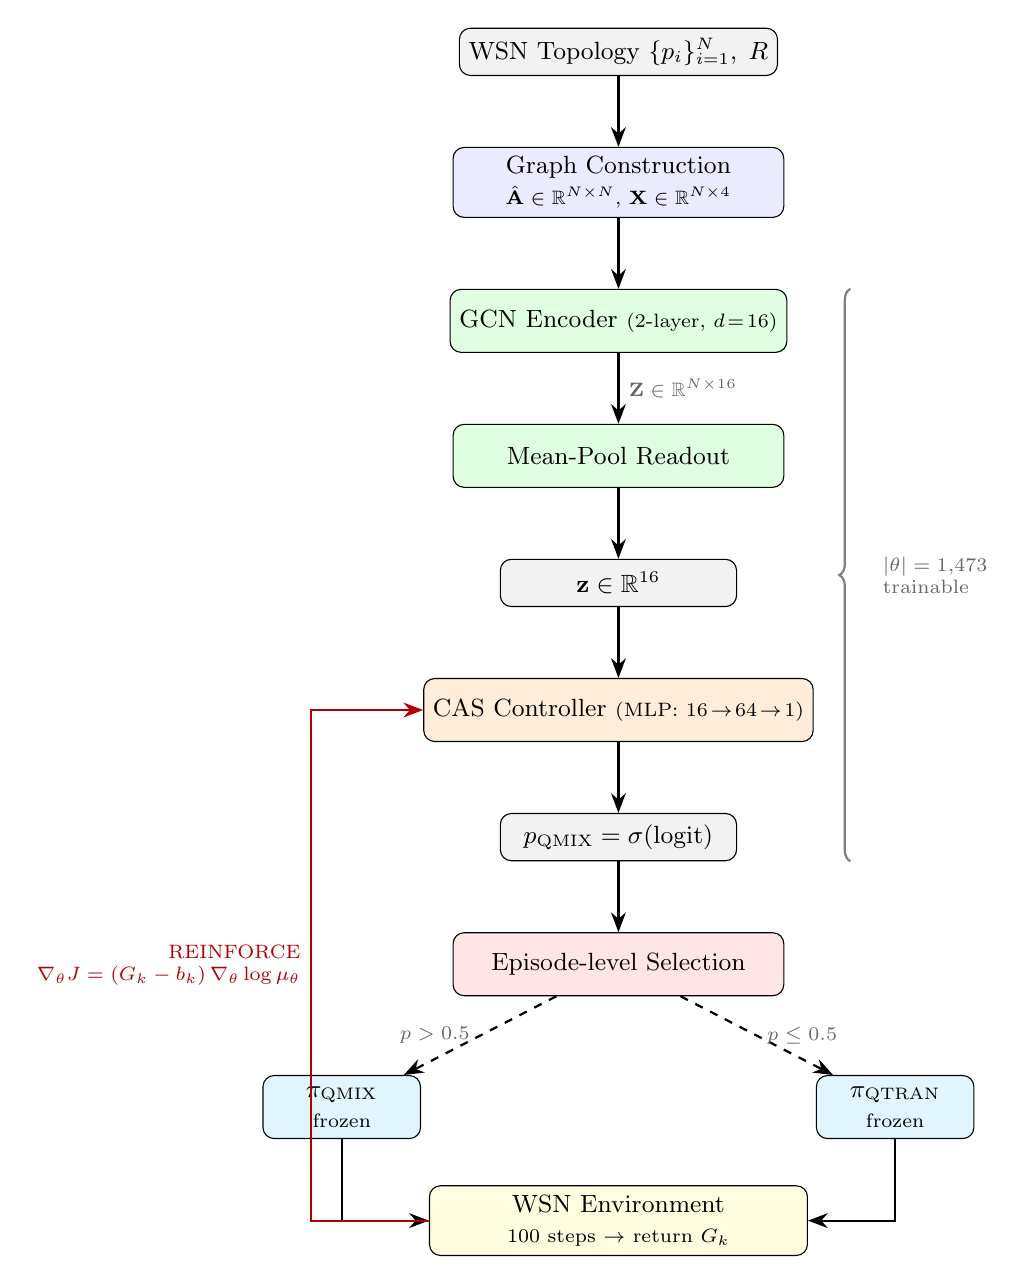
\begin{tikzpicture}[
    node distance=0.9cm,
    box/.style={draw, rounded corners, minimum height=0.8cm, minimum width=4.2cm, align=center, font=\small},
    data/.style={draw, rounded corners, minimum height=0.6cm, minimum width=3.0cm, align=center, fill=gray!10, font=\small},
    arrow/.style={-{Stealth[length=2.5mm]}, thick},
    dasharrow/.style={-{Stealth[length=2.5mm]}, thick, dashed},
    label/.style={font=\scriptsize, text=black!60},
]
\node[data] (topo) {WSN Topology $\{p_i\}_{i=1}^N,\; R$};
\node[box, below=of topo, fill=blue!8] (graph) {Graph Construction\\{\scriptsize $\hat{\mathbf{A}} \in \mathbb{R}^{N \times N}$, $\mathbf{X} \in \mathbb{R}^{N \times 4}$}};
\node[box, below=of graph, fill=green!12] (gcn) {GCN Encoder {\scriptsize (2-layer, $d\!=\!16$)}};
\node[box, below=of gcn, fill=green!12] (pool) {Mean-Pool Readout};
\node[data, below=of pool] (embed) {$\mathbf{z} \in \mathbb{R}^{16}$};
\node[box, below=of embed, fill=orange!15] (cas) {CAS Controller {\scriptsize (MLP: $16 \!\to\! 64 \!\to\! 1$)}};
\node[data, below=of cas] (prob) {$p_{\text{QMIX}} = \sigma(\text{logit})$};
\node[box, below=of prob, fill=red!10] (decision) {Episode-level Selection};
\node[box, below left=1.0cm and 0.4cm of decision, fill=cyan!12, minimum width=2.0cm] (qmix) {$\pi_{\text{QMIX}}$\\{\scriptsize frozen}};
\node[box, below right=1.0cm and 0.4cm of decision, fill=cyan!12, minimum width=2.0cm] (qtran) {$\pi_{\text{QTRAN}}$\\{\scriptsize frozen}};
\node[box, below=2.4cm of decision, fill=yellow!12, minimum width=4.8cm] (env) {WSN Environment\\{\scriptsize 100 steps $\to$ return $G_k$}};
\draw[arrow] (topo) -- (graph);
\draw[arrow] (graph) -- (gcn);
\draw[arrow] (gcn) -- node[right, label] {$\mathbf{Z} \in \mathbb{R}^{N \times 16}$} (pool);
\draw[arrow] (pool) -- (embed);
\draw[arrow] (embed) -- (cas);
\draw[arrow] (cas) -- (prob);
\draw[arrow] (prob) -- (decision);
\draw[dasharrow] (decision) -- node[left, label] {$p > 0.5$} (qmix);
\draw[dasharrow] (decision) -- node[right, label] {$p \leq 0.5$} (qtran);
\draw[arrow] (qmix) |- (env);
\draw[arrow] (qtran) |- (env);
\draw[arrow, red!70!black, thick]
    (env.west) -- ++(-1.5, 0) |- (cas.west)
    node[pos=0.25, left, font=\scriptsize, text=red!70!black, align=right]
    {REINFORCE\\$\nabla_\theta J = (G_k - b_k)\,\nabla_\theta \log \mu_\theta$};
\draw[decorate, decoration={brace, amplitude=4pt, mirror}, thick, black!50]
    let \p1=(gcn.north east), \p2=(prob.south east) in
    (\x1+0.8cm, \y1) -- (\x1+0.8cm, \y2)
    node[midway, right=8pt, font=\scriptsize, text=black!60, align=left] 
    {$|\theta| = 1{,}473$\\trainable};
\end{tikzpicture}
}
\captionof{figure}{GAPF architecture (CAS mode). Sensor positions and communication radius define a graph encoded by a two-layer GCN with mean-pool readout ($\mathbf{z} \in \mathbb{R}^{16}$). The CAS controller maps $\mathbf{z}$ to a selection probability $p_{\text{QMIX}}$. The chosen frozen expert executes the full episode. The return $G_k$ feeds back (red arrow) as a REINFORCE signal to update only the $1{,}473$ meta-controller parameters.}
\label{fig:gapf_architecture}
\end{center}

\subsubsection{Training Procedure}
\label{sec:gapf_training}

QMIX and QTRAN are trained independently; their parameters are then frozen. Only the GAPF meta-controller ($1{,}473$ parameters) is trained via REINFORCE~\cite{williams1992simple} with an EMA baseline. Let $G_k$ denote the episodic return from executing the selected expert $\pi_{a^{\text{meta}}_k}$ in episode~$k$. The policy gradient is:
\begin{equation}
    \nabla_\theta J(\theta) = \mathbb{E}\!\left[\left(G_k - b_k\right) \nabla_\theta \log \mu_\theta\!\left(a^{\text{meta}}_k \mid \mathcal{G}_k\right)\right],
    \label{eq:reinforce}
\end{equation}
where $b_k$ is the EMA baseline updated as $b_{k+1} = 0.95\, b_k + 0.05\, G_k$. Since the selection is Bernoulli, $\log \mu_\theta = \log p_{\text{QMIX}}$ if QMIX is chosen and $\log(1 - p_{\text{QMIX}})$ otherwise. Parameters are updated via Adam with learning rate $\alpha = 3 \times 10^{-3}$ and gradient clipping $\|\nabla_\theta\|_2 \leq 1.0$. The complete procedure is summarised in Algorithm~\ref{alg:gapf_training}.

\begin{algorithm}[H]
\caption{GAPF Training --- Pseudocode (CAS Mode)}
\label{alg:gapf_training}
\begin{algorithmic}[1]
\REQUIRE Frozen expert policies $\pi_{\text{QMIX}}$, $\pi_{\text{QTRAN}}$; WSN environment $\mathcal{M}$; training episodes $K$
\ENSURE Trained meta-controller parameters $\theta$
\STATE \COMMENT{--- Initialisation ---}
\STATE Initialise $\theta$ using Xavier uniform distribution
\STATE Create Adam optimiser with learning rate $\alpha = 3 \times 10^{-3}$
\STATE $b \leftarrow \text{None}$ \COMMENT{EMA baseline for variance reduction}
\FOR{$k = 1, \ldots, K$}
    \STATE \COMMENT{--- Topology encoding (once per episode) ---}
    \STATE Reset $\mathcal{M}$; obtain sensor positions $\{p_i\}$ and radius $R$
    \STATE $(\hat{\mathbf{A}}_k, \mathbf{X}_k) \leftarrow$ Algorithm~\ref{alg:graph_construction} applied to $(\{p_i\}, p_{\text{BS}}, R, L)$
    \STATE $\mathbf{H} \leftarrow \text{ReLU}(\hat{\mathbf{A}}_k \cdot \mathbf{X}_k \cdot \mathbf{W}_1)$ \COMMENT{GCN layer 1}
    \STATE $\mathbf{Z} \leftarrow \hat{\mathbf{A}}_k \cdot \mathbf{H} \cdot \mathbf{W}_2$ \COMMENT{GCN layer 2}
    \STATE $\mathbf{z}_k \leftarrow \frac{1}{N}\sum_{i=1}^{N} \mathbf{Z}_{i,:}$ \COMMENT{Mean-pool graph embedding}
    \STATE \COMMENT{--- Expert selection (stochastic during training) ---}
    \STATE $p_{\text{QMIX}} \leftarrow \sigma(\mathbf{w}_2^\top \cdot \text{ReLU}(\mathbf{W}_c \cdot \mathbf{z}_k + \mathbf{b}_c) + b_2)$ \COMMENT{CAS probability}
    \STATE Sample $a^{\text{meta}}_k \sim \text{Bernoulli}(p_{\text{QMIX}})$ \COMMENT{$1 \to$ QMIX, $0 \to$ QTRAN}
    \STATE Execute expert $\pi_{a^{\text{meta}}_k}$ for $T$ steps; collect episodic return $G_k$
    \STATE \COMMENT{--- REINFORCE update with EMA baseline ---}
    \IF{$b = \text{None}$}
        \STATE $b \leftarrow G_k$ \COMMENT{Initialise baseline with first return}
    \ENDIF
    \STATE $\delta_k \leftarrow G_k - b$ \COMMENT{Advantage estimate}
    \STATE $b \leftarrow 0.95 \cdot b + 0.05 \cdot G_k$ \COMMENT{Update EMA baseline}
    \STATE \COMMENT{Skip update if advantage is near zero}
    \IF{$|\delta_k| > 10^{-8}$}
        \STATE $\mathcal{L} \leftarrow -\delta_k \cdot \log \mu_\theta(a^{\text{meta}}_k \mid \mathcal{G}_k)$ \COMMENT{Policy gradient loss}
        \STATE Clip gradients: $\|\nabla_\theta \mathcal{L}\|_2 \leq 1.0$
        \STATE Update $\theta$ via Adam
    \ENDIF
\ENDFOR
\RETURN $\theta$
\end{algorithmic}
\end{algorithm}

Algorithm~\ref{alg:gapf_execution} describes the full inference-time procedure used during evaluation and deployment.

\begin{algorithm}[H]
\caption{GAPF Episode Execution --- Pseudocode (Inference)}
\label{alg:gapf_execution}
\begin{algorithmic}[1]
\REQUIRE Trained meta-controller $\mu_\theta$; frozen experts $\pi_{\text{QMIX}}$, $\pi_{\text{QTRAN}}$; environment $\mathcal{M}$; episode length $T$
\ENSURE Episodic return $G$, routing metrics (PDR, $E_{\text{tot}}$, $\sigma_E$)
\STATE \COMMENT{--- Phase 1: Topology encoding (executed once per episode) ---}
\STATE Reset $\mathcal{M}$; obtain sensor positions $\{p_i\}_{i=1}^N$ and radius $R$
\STATE $(\hat{\mathbf{A}}, \mathbf{X}) \leftarrow$ Algorithm~\ref{alg:graph_construction} applied to $(\{p_i\}, p_{\text{BS}}, R, L)$
\STATE $\mathbf{H} \leftarrow \text{ReLU}(\hat{\mathbf{A}} \cdot \mathbf{X} \cdot \mathbf{W}_1)$ \COMMENT{GCN layer 1: neighbour aggregation}
\STATE $\mathbf{Z} \leftarrow \hat{\mathbf{A}} \cdot \mathbf{H} \cdot \mathbf{W}_2$ \COMMENT{GCN layer 2}
\STATE $\mathbf{z} \leftarrow \frac{1}{N} \sum_{i=1}^{N} \mathbf{Z}_{i,:}$ \COMMENT{Mean-pool readout $\to \mathbf{z} \in \mathbb{R}^{16}$}
\STATE \COMMENT{--- Phase 2: Expert selection via CAS controller ---}
\STATE $p_{\text{QMIX}} \leftarrow \sigma\!\left(\mathbf{w}_2^\top \cdot \text{ReLU}(\mathbf{W}_c \cdot \mathbf{z} + \mathbf{b}_c) + b_2\right)$ \COMMENT{Selection probability}
\IF{$p_{\text{QMIX}} > 0.5$}
    \STATE SelectedExpert $\leftarrow \pi_{\text{QMIX}}$
\ELSE
    \STATE SelectedExpert $\leftarrow \pi_{\text{QTRAN}}$
\ENDIF
\STATE \COMMENT{--- Phase 3: Decentralised step-by-step execution ---}
\STATE Initialise hidden states $\mathbf{h}_i^{(0)} \leftarrow \mathbf{0}$ for all agents $i$
\STATE $G \leftarrow 0$
\FOR{$t = 1, \ldots, T$}
    \FOR{each agent $i = 1, \ldots, N$}
        \STATE Observe local state $\mathbf{o}_i^{(t)} \leftarrow [RE_i,\, CE_i,\, x_i,\, y_i,\, N_i]$ \COMMENT{5-dim observation}
        \STATE $(\mathbf{q}_i,\, \mathbf{h}_i^{(t)}) \leftarrow$ SelectedExpert$(\mathbf{o}_i^{(t)},\, \mathbf{h}_i^{(t-1)})$ \COMMENT{GRU forward pass}
        \STATE Set $q_{ij} \leftarrow -\infty$ for out-of-range or energy-depleted neighbour $j$ \COMMENT{Valid-action mask}
        \STATE $a_i^{(t)} \leftarrow \argmax_j \mathbf{q}_i[j]$ \COMMENT{Greedy action selection}
    \ENDFOR
    \STATE Execute joint action $(a_1^{(t)}, \ldots, a_N^{(t)})$ in $\mathcal{M}$
    \STATE Collect rewards $\{r_i^{(t)}\}$; update environment state
    \STATE $G \leftarrow G + \sum_{i=1}^{N} r_i^{(t)}$
\ENDFOR
\STATE Compute final metrics: PDR, $E_{\text{tot}}$, $\sigma_E$ from environment state
\RETURN $G$, PDR, $E_{\text{tot}}$, $\sigma_E$
\end{algorithmic}
\end{algorithm}


\subsubsection{Design Rationale}
\label{sec:gapf_rationale}

Five design choices distinguish GAPF from standard ensemble methods and recent mixture-of-experts RL architectures~\cite{yang_pamoe_2026}: \textbf{(1)}~\emph{Topology awareness}: the GCN encodes the spatial graph, allowing the controller to learn that certain topologies favour one expert over another. \textbf{(2)}~\emph{Episode-level granularity}: selection occurs once per episode, avoiding instability from switching experts mid-episode where GRU-based agents have incompatible hidden state dynamics. \textbf{(3)}~\emph{Minimal overhead}: $1{,}473$ parameters vs.\ $38{,}983$ per expert; the GCN runs once per episode and the CAS decision is a single MLP forward pass. \textbf{(4)}~\emph{Frozen experts}: pre-trained policies are not fine-tuned, preserving validated performance and reducing the optimisation landscape to $1{,}473$ dimensions. \textbf{(5)}~\emph{Deployment feasibility}: each agent's GRU ($38{,}983$ parameters $\approx 38$\,KB in int8 quantisation) fits within typical WSN microcontroller RAM (nRF52840: 256\,KB; ESP32: 520\,KB), enabling on-device inference.

\subsubsection{Comparison with Alternative Lightweight Approaches}
\label{sec:comparison_alternatives}

Strategies based on node-degree or local graph metrics (clustering coefficient, betweenness centrality) operate on \emph{pre-defined, single-hop} structural features that cannot encode higher-order topological patterns such as bottleneck corridors or multi-hop connectivity islands. In contrast, GAPF's two-layer GCN propagates information across each node's 2-hop neighbourhood, producing a graph-level embedding $\mathbf{z} \in \mathbb{R}^{16}$ that captures global connectivity structure; notably, node-degree is already one of the four input features (Eq.~\ref{eq:node_features}), which the GCN \emph{enriches} through aggregation. Fuzzy inference systems (e.g., QPSOFL's Mamdani-type controller) require manual specification of linguistic variables, membership functions, and rule bases---a topology-specific process that does not transfer across configurations without re-tuning. GAPF avoids this feature engineering bottleneck: its GCN weights are learned end-to-end via REINFORCE and generalise across 7 scenarios (20--100 sensors, 25--50\,m radius) at $\geq$98\% PDR without per-scenario tuning, whereas QPSOFL collapses below 15\% PDR in sparse topologies. The GCN's per-episode overhead ($\mathcal{O}(n^2 d)$, $d{=}16$, $<0.03$\,ms) is negligible relative to per-step routing costs.

\subsubsection{Meta-Learning Architecture vs.\ End-to-End Multi-Agent DRL}
\label{sec:meta_vs_e2e}

GAPF's two-stage design (pre-trained frozen experts $+$ lightweight meta-controller) contrasts with end-to-end multi-agent DRL along three dimensions. \emph{Learning dynamics}: end-to-end MARL must simultaneously optimise agent policies, value decomposition, and implicit topology adaptation through a single gradient signal, creating a non-stationary problem where each agent's optimal policy depends on every other agent's changing policy; GAPF separates these concerns---experts converge independently, and the 1{,}473-parameter meta-controller solves the simpler problem of mapping topology embeddings to binary selection, converging in ${\sim}2{,}000$ episodes versus ${\sim}200{,}000$ steps per expert. \emph{Memory}: the dominant cost in end-to-end MARL is the replay buffer ($15{,}000$ episodes $\times$ $n$ agents); GAPF trains on-policy and eliminates this entirely, yielding a $13\times$ reduction in peak RAM (Table~\ref{tab:consolidated_balance}) and passing the 1{,}024\,MB constraint that standalone QMIX/QTRAN fail in every scenario. \emph{Per-step computation}: at execution time, GAPF's per-step cost is identical to standalone QMIX or QTRAN ($\mathcal{O}(n^2 h + nh^2)$); the GCN adds only a one-time $\mathcal{O}(n^2 d)$ cost amortised over $T{=}100$ steps.

Here is the complete time-complexity analysis. 
\subsection{Time Complexity Analysis}
\label{sec:complexity}

Let $n$ denote the number of sensor agents, $h = 64$ the RNN hidden dimension, $d = 16$ the GNN embedding dimension, and $T$ the number of steps per episode.

At each routing step, only the frozen expert executes; across all $n$ agents the per-step cost is $\mathcal{O}_{\text{step}} = \mathcal{O}(n^2 h + n h^2)$, \textbf{identical for QMIX, QTRAN, and GAPF}. GAPF adds a one-time per-episode overhead for adjacency construction ($\mathcal{O}(n^2)$), a two-layer GCN forward pass ($\mathcal{O}(n^2 d + n d^2)$), and the CAS MLP ($\mathcal{O}(dm)$), yielding $\mathcal{O}_{\text{GAPF-init}} = \mathcal{O}(n^2 d)$. For an episode of $T$ steps the total is $\mathcal{O}(Tn^2 h + Tnh^2 + n^2 d)$; since $Th \gg d$ the GCN overhead is amortised and the dominant term $\mathcal{O}(Tn^2 h)$ matches standalone QMIX/QTRAN.

\begin{center}
\captionof{table}{Time complexity comparison. $n$: number of sensors, $T$: steps per episode, $h$: RNN hidden dimension (64), $d$: GNN embedding dimension (16), $N_p$: PSO particles (32), $I$: PSO iterations (50).}
\label{tab:complexity}
\begin{tabular}{lcc}
\toprule
Algorithm & Per-Step & Per-Episode \\
\midrule
QMIX / QTRAN & $\mathcal{O}(n^2 h + n h^2)$ & $\mathcal{O}(T(n^2 h + n h^2))$ \\
QPSOFL  & $\mathcal{O}(N_p \cdot n^2)$ & $\mathcal{O}(T \cdot I \cdot N_p \cdot n^2)$ \\
\textbf{GAPF} & $\mathcal{O}(n^2 h + n h^2)$ & $\mathcal{O}(T(n^2 h + n h^2) + n^2 d)$ \\
\bottomrule
\end{tabular}
\end{center}

\noindent GAPF adds only $\mathcal{O}(n^2 d)$ per episode, where $d = 16 \ll h = 64$, making its per-step complexity identical to standalone QMIX/QTRAN. In contrast, QPSOFL's cost grows as $\mathcal{O}(T \cdot I \cdot N_p \cdot n^2)$ due to repeated swarm optimisation at every step, explaining its longer wall-clock times despite having no neural network.



\section{Results and Discussion}

Table~\ref{table_setting} presents the custom Gym environment setting.

\begin{center}
\captionof{table}{Custom Gym Environment setting.}
\label{table_setting}
\resizebox{0.6\textwidth}{!}{
\begin{tabular}{|>{\columncolor{gray!50}}c|>{\columncolor{gray!10}}c|}
\hline
\textbf{Key} & \textbf{Value} \\
\hline
$E_{\text{elec}}$ & $50 \times 10^{-9}$ J/bit \\
\hline
$E_{\text{amp}}$ & $100 \times 10^{-12}$ J/(bit$\cdot$m$^2$) \\
\hline
Packet size & 512 bit \\
\hline
Initial energy per sensor ($E_0$) & 1 J \\
\hline
Field bounds (LowerBound, UpperBound) & 0--100 m \\
\hline
Base station position & (50, 50) \\
\hline
Initial packets per sensor & 1 \\
\hline
Total timesteps / Max per episode & 200,000 / 100 \\
\hline
\end{tabular}
}
\end{center}

Table~\ref{tab:hyperparameters} displays the training hyperparameters. QMIX and QTRAN are trained independently as separate expert policies; their parameters are then frozen, and only the lightweight GAPF meta-controller (${\sim}1{,}473$ parameters) is trained to dynamically select between them based on network topology.

\begin{center}
\captionof{table}{Training Hyperparameters for QMIX, QTRAN, and GAPF.}
\label{tab:hyperparameters}
\resizebox{\textwidth}{!}{
\begin{tabular}{llccc}
\toprule
\textbf{Category} & \textbf{Parameter} & \textbf{QMIX} & \textbf{QTRAN} & \textbf{GAPF} \\
\midrule
\multirow{3}{*}{Optimization}
& Optimizer / LR       & Adam / 0.0003 & RMSprop / 0.0003 & Adam / 0.003 \\
& Grad clip / $\gamma$ & 10 / 0.99     & 10 / 0.99        & 1.0 / ---    \\
& Reward scale         & 0.01          & 0.01             & ---          \\
\midrule
\multirow{2}{*}{Exploration}
& Strategy             & $\varepsilon$-greedy & $\varepsilon$-greedy & REINFORCE \\
& $\varepsilon$: start$\to$end (anneal) & $0.5\to0.01$ (150K) & $0.5\to0.01$ (150K) & --- \\
\midrule
\multirow{2}{*}{Architecture}
& Agent / hidden dim   & GRU(64) / 64  & GRU(64) / 64  & GCN+MLP / 16+64 \\
& Mixing embed dim     & 64            & 64             & ---              \\
\midrule
\multirow{3}{*}{Training}
& Episodes / batch     & ${\sim}$2K / 32 & ${\sim}$2K / 32 & 2K / 1 (on-policy) \\
& Replay buffer        & 15,000       & 15,000        & ---              \\
& Target update        & Hard, every 30 ep. & Hard, every 30 ep. & EMA $\beta{=}0.95$ \\
\midrule
QTRAN-specific & $\lambda_{\text{opt}}$ / $\lambda_{\text{nopt}}$ & --- & 1.0 / 0.1 & --- \\
\midrule
Evaluation & Test episodes / eval $\varepsilon$ & 1,000 / 0.01 & 1,000 / 0.01 & 1,000 / --- \\
\bottomrule
\end{tabular}
}
\end{center}

Our evaluation includes QPSOFL~\cite{hu_energy_2024}, a metaheuristic baseline using Quantum PSO with Sobol-initialized particles and L'evy flight for cluster-head selection, followed by Mamdani-type Fuzzy Inference for relay selection.

\paragraph{Execution-time instrumentation.}
The framework records per-step wall-clock times (mean, p95, p99) as versioned \texttt{.npy} arrays. A standalone benchmark tool measures latency over 30 iterations (3 warmup), peak RAM via \texttt{tracemalloc}, analytical MACs/FLOPs, and estimated energy per inference ($\mu$J). Table~\ref{tab:reviewer7_latency} reports results for the worst case ($N{=}70$).

\begin{center}
\captionof{table}{Inference metrics (Apple M-series CPU, 0.1,W reference). All algorithms achieve sub-millisecond latency.}
\label{tab:reviewer7_latency}
\renewcommand{\arraystretch}{1.15}
\begin{tabular}{@{}lcccc@{}}
\toprule
\textbf{Algorithm} & \textbf{Latency p95 (ms)} & \textbf{Peak RAM (KB)} & \textbf{MACs} & \textbf{Energy ($\mu$J)} \\
\midrule
QMIX (agent + mixer)   & 0.27 & 2.98  & 2{,}539{,}904 & 27.2 \\
QTRAN (agent + mixer)   & 0.17 & 34.32 & 4{,}955{,}532 & 16.7 \\
GAPF (GCN, gateway)     & 0.03 & 4.12  & 181{,}408     & 3.0  \\
\midrule
Agent only (deployed)    & $<$1 & $\sim$2 & $\sim$29K  & $<$10 \\
\bottomrule
\end{tabular}
\end{center}

Even scaling by $50\times$ for a resource-constrained ARM Cortex-M4 at 80,MHz, the per-step decision time remains under 15,ms---well within real-time WSN budgets.

Seven scenarios (Table~\ref{tab:scenarios}) systematically vary network density ($n$) and coverage radius ($R$), each evaluated over three random seeds (42, 123, 456).

\begin{center}
\captionof{table}{Overview of the seven evaluation scenarios.}
\label{tab:scenarios}
\begin{tabular}{cccl}
\hline
\textbf{\#} & $n$ & $R$ (m) & \textbf{Rationale} \\
\hline
1 & 20  & 25 & Sparse, short range --- extreme connectivity challenge \\
2 & 30  & 25 & Small--medium, short range --- limited relay options \\
3 & 50  & 35 & Medium, standard range --- moderate density \\
4 & 70  & 35 & Baseline --- dense, standard range \\
5 & 70  & 45 & Dense, extended range --- more routing options \\
6 & 100 & 35 & Large-scale, standard range --- scalability test \\
7 & 100 & 50 & Large-scale, long range --- high connectivity stress \\
\hline
\end{tabular}
\end{center}

\subsubsection{Consolidated Results Across All Scenarios}

Table~\ref{tab:consolidated_perf} presents key performance metrics for all seven scenarios. All values are mean $\pm$ std aggregated over three seeds on the 1{,}000-episode test set. PDR denotes packet delivery ratio, $E_{\text{tot}}$ total energy consumed (J), $\sigma_{E}$ standard deviation of remaining energy (lower is better balanced), and Throughput is packets delivered per step.

\begin{center}
\captionof{table}{Performance metrics across all scenarios (three seeds, test set). Best values per scenario in \textbf{bold}.}
\label{tab:consolidated_perf}
\resizebox{\textwidth}{!}{
\begin{tabular}{cc|cccc|cccc}
\toprule
& & \multicolumn{4}{c|}{\textbf{PDR}} & \multicolumn{4}{c}{\textbf{$E_{\text{tot}}$ (J)}} \\
$n$ & $R$ & QMIX & QTRAN & QPSOFL & \textbf{GAPF} & QMIX & QTRAN & QPSOFL & \textbf{GAPF} \\
\midrule
20  & 25 & $.559\pm.257$ & $.558\pm.258$ & $.075\pm.107$ & $\mathbf{.753\pm.161}$ & $.093\pm.055$ & $.093\pm.055$ & $\mathbf{.052\pm.049}$ & $.075\pm.044$ \\
30  & 25 & $.568\pm.179$ & $.567\pm.174$ & $.053\pm.046$ & $\mathbf{.877\pm.159}$ & $.165\pm.054$ & $.166\pm.054$ & $\mathbf{.102\pm.050}$ & $.102\pm.070$ \\
50  & 35 & $.553\pm.248$ & $.552\pm.250$ & $.153\pm.092$ & $\mathbf{.990\pm.088}$ & $.423\pm.152$ & $.422\pm.153$ & $\mathbf{.113\pm.072}$ & $.202\pm.131$ \\
70  & 35 & $.545\pm.242$ & $.545\pm.243$ & $.122\pm.090$ & $\mathbf{.980\pm.119}$ & $.600\pm.204$ & $.603\pm.200$ & $\mathbf{.198\pm.116}$ & $.283\pm.213$ \\
70  & 45 & $.667\pm.246$ & $.659\pm.256$ & $.365\pm.092$ & $\mathbf{.980\pm.124}$ & $.687\pm.265$ & $.692\pm.274$ & $\mathbf{.040\pm.040}$ & $.334\pm.272$ \\
100 & 35 & $.464\pm.270$ & $.462\pm.261$ & $.099\pm.080$ & $\mathbf{.980\pm.124}$ & $1.010\pm.295$ & $1.017\pm.282$ & $\mathbf{.312\pm.171}$ & $.334\pm.272$ \\
100 & 50 & $.669\pm.266$ & $.684\pm.270$ & $.448\pm.057$ & $\mathbf{.980\pm.124}$ & $1.181\pm.413$ & $1.180\pm.412$ & $\mathbf{.026\pm.025}$ & $.334\pm.272$ \\
\bottomrule
\end{tabular}
}
\end{center}

\begin{center}
\captionof{table}{Energy balance ($\sigma_E$) and feasibility compliance across all scenarios.}
\label{tab:consolidated_balance}
\resizebox{\textwidth}{!}{
\begin{tabular}{cc|cccc|cc|cc}
\toprule
& & \multicolumn{4}{c|}{$\sigma_E$ (lower = better)} & \multicolumn{2}{c|}{Memory $<1024$,MB?} & \multicolumn{2}{c}{$p_{99}<50$,ms?} \\
$n$ & $R$ & QMIX & QTRAN & QPSOFL & \textbf{GAPF} & QMIX/QTRAN & GAPF & QMIX/QTRAN & GAPF \\
\midrule
20  & 25 & .0075 & .0075 & .0056 & $\mathbf{.0043}$ & FAIL & PASS & PASS & PASS \\
30  & 25 & .0111 & .0112 & .0085 & $\mathbf{.0035}$ & FAIL & PASS & PASS & PASS \\
50  & 35 & .0264 & .0265 & .0081 & $\mathbf{.0039}$ & FAIL & PASS & PASS & PASS \\
70  & 35 & .0318 & .0319 & .0114 & $\mathbf{.0049}$ & FAIL & PASS & PASS & PASS \\
70  & 45 & .0379 & .0382 & $\mathbf{.0024}$ & .0061 & FAIL & PASS & PASS & PASS \\
100 & 35 & .0455 & .0457 & .0144 & $\mathbf{.0061}$ & FAIL & PASS & PASS & PASS \\
100 & 50 & .0559 & .0559 & $\mathbf{.0010}$ & .0061 & FAIL & PASS & PASS & PASS \\
\bottomrule
\end{tabular}
}
\end{center}

\subsubsection{Key Findings}

Five principal findings emerge from the seven scenarios:

\paragraph{(F1) GAPF consistently achieves the highest PDR, with the advantage growing in sparser networks.}
GAPF's relative PDR improvement over the best standalone MARL baseline scales from $+35\%$ ($n{=}20$) to $+54\%$ ($n{=}30$), $+79\%$ ($n{=}50$), and peaks at $+111\%$ ($n{=}100$, $R{=}35$). Increasing the coverage radius narrows the gap (e.g., $+80\%$ at $(70,35)$ vs $+47\%$ at $(70,45)$; $+111\%$ at $(100,35)$ vs $+43\%$ at $(100,50)$), confirming that GAPF's topology-aware policy fusion is most valuable where routing is hardest---sparse networks with limited relay options.

\paragraph{(F2) GAPF achieves $2$--$3.5\times$ lower energy consumption and $3$--$9\times$ better energy balance than QMIX/QTRAN.}
While QPSOFL uses the least total energy in most scenarios, its near-zero delivery renders this meaningless. Among algorithms with viable PDR ($>50\%$), GAPF consistently uses the least energy. The energy balance ratio ($\sigma_E^{\text{QMIX}}/\sigma_E^{\text{GAPF}}$) widens from $1.7\times$ ($n{=}20$) to $9.2\times$ ($n{=}100$, $R{=}50$), confirming that GAPF's GCN-based load distribution scales with network size.

\paragraph{(F3) QMIX and QTRAN converge to statistically indistinguishable performance.}
Across all scenarios, QMIX and QTRAN yield nearly identical PDR (within 1--2\%), energy, and latency. This validates GAPF's design: the performance gain stems from the GCN-based topology-aware controller and policy fusion, not from expert selection alone.

\paragraph{(F4) QPSOFL collapses at scale; low energy reflects non-delivery.}
QPSOFL's PDR degrades from $7.5\%$ ($n{=}20$) to below $10\%$ at $n{=}100$, $R{=}35$. Wider coverage radii partially recover delivery ($44.8\%$ at $n{=}100$, $R{=}50$), but performance remains unacceptable. Its excellent energy balance at high $R$ (e.g., $\sigma_E{=}0.001$ at $(100,50)$) is an artifact of minimal packet transmission rather than intelligent routing.

\paragraph{(F5) GAPF is the only algorithm passing all feasibility constraints.}
QMIX/QTRAN \textbf{fail} the 1{,}024,MB memory constraint in every scenario (peak memory $3.2$--$13.8$,GB), while GAPF stays within budget ($684$--$951$,MB). All algorithms pass the $p_{99}{<}50$,ms latency constraint. GAPF's memory footprint at $n{=}100$ ($951$,MB) leaves only $7\%$ headroom, warranting attention for even larger deployments.

\subsection{Deployment Feasibility on Resource-Constrained Nodes}
\label{sec:deployment_feasibility}

The CTDE paradigm~\cite{kraemer2016multi,lowe2017multi} decouples training from deployment complexity. At inference time, the heavy training-only components---value-decomposition mixers, reward scalarization network, ES loop---are \emph{discarded entirely}.

\begin{center}
\captionof{table}{Component deployment map under CTDE. Only the per-sensor agent and GAPF controller are active at inference.}
\label{tab:deployment_components}
\renewcommand{\arraystretch}{1.15}
\resizebox{\textwidth}{!}{
\begin{tabular}{@{}lccc@{}}
\toprule
\textbf{Component} & \textbf{Runs on} & \textbf{Deployed?} & \textbf{Size} \\
\midrule
QMIX/QTRAN mixer, Q$\cdot$K Attention, ES loop & Training server & No & --- \\
\midrule
GAPF meta-controller (GCN + CAS) & Sink/gateway & Yes (1$\times$/episode) & $\sim$1{,}473 params ($\sim$6,KB) \\
Per-sensor agent (GRU) & Each sensor & Yes (1$\times$/step) & $\sim$25K params ($\sim$100,KB) \\
\bottomrule
\end{tabular}
}
\end{center}

Each sensor executes a single-layer GRU agent:
\begin{equation}
a_i = \argmax_{j}; \mathbf{W}_2 ;\mathrm{GRU}!\bigl(\mathrm{ReLU}(\mathbf{W}_1 \mathbf{o}_i + \mathbf{b}1),; \mathbf{h}{i}^{(t-1)}\bigr) + \mathbf{b}_2
\label{eq:agent_forward}
\end{equation}
where $\mathbf{o}_i \in \mathbb{R}^5$ is the local observation (remaining energy, consumed energy, $x$-$y$ position, packet count), $\mathbf{h}_i^{(t-1)} \in \mathbb{R}^{64}$ is the recurrent hidden state, and $|\mathcal{A}|{=}N{+}1$. A single forward pass requires ${\sim}29$K MACs (${\sim}320$ for the input layer, ${\sim}24{,}576$ for the GRU cell, ${\sim}4{,}544$ for the output layer at $n{=}70$), which completes in $<1$,ms even on an ARM Cortex-M4 at 80,MHz. The full model fits in ${\sim}100$,KB of flash, well within the capacity of commercial WSN platforms such as the STM32L4 (1,MB flash, 320,KB SRAM) or nRF52840 (1,MB flash, 256,KB RAM).

\subsection{Limitations}
\label{sec:limitations}

Despite GAPF's strong empirical performance, several limitations warrant discussion:

\begin{enumerate}
    \item \textbf{Simulation-only validation.} All experiments are conducted in a custom OpenAI Gym simulator. While we provide deployment feasibility analysis (Section~\ref{sec:deployment_feasibility}) showing that the deployed agent requires only ${\sim}100$ lines of C and $<30$\,\textmu J per inference on a Cortex-M4 MCU, no hardware-in-the-loop experiments have been performed. Real-world factors such as channel fading, packet collisions, and clock drift are not modelled.
    
    \item \textbf{Static topology assumption.} GAPF computes the graph embedding once per episode and selects a fixed expert for the entire episode. In scenarios with mobile sensors or rapidly changing channel conditions, step-level re-evaluation may be necessary. Three extensions can address this, ordered by complexity: (i)~\emph{periodic re-evaluation} every $K$ steps with GRU hidden state reset (overhead: $\lceil T/K \rceil \times 0.03$\,ms); (ii)~\emph{confidence-triggered re-evaluation} when $|p_{\text{QMIX}} - 0.5| < \delta$; and (iii)~\emph{step-level Q-value fusion} blending both experts' outputs via a learned weight $\alpha_t$ at the cost of doubled per-step computation. In practice, WSN topologies change on the order of minutes to hours while a routing episode spans seconds, making option~(i) sufficient for most deployments.
    
    \item \textbf{Two-expert limitation.} The current CAS controller produces a binary selection (QMIX vs QTRAN). Extending to $k > 2$ experts (e.g., incorporating DQN, MAPPO, or QPLEX) would require a softmax-based selection mechanism and raises questions about diminishing returns as expert diversity increases.
    
    \item \textbf{Fixed episode length.} All scenarios use $T = 100$ steps per episode. Real WSN deployments operate continuously with time-varying traffic patterns and gradual energy depletion over days or weeks. The episodic formulation does not capture long-horizon energy management.
    
    \item \textbf{Memory constraint tightness.} At $n{=}100$, GAPF's memory footprint reaches 951\,MB---within the 1\,GB constraint but with only 7\% headroom. Scaling beyond $n{=}100$ may require model compression techniques (pruning, quantisation) to remain feasible on resource-constrained gateways.
    
    \item \textbf{Homogeneous sensor assumption.} All sensors are identical in hardware capability and initial energy. Heterogeneous deployments with mixed sensor types, varying transmission power, or asymmetric energy budgets are not evaluated. However, the architecture accommodates heterogeneity with minimal changes: the node feature vector (Eq.~\ref{eq:node_features}) extends from $\mathbb{R}^4$ to $\mathbb{R}^{4+k}$ by appending sensor-specific attributes (battery capacity, transmission power, sensor type), requiring only a resized $\mathbf{W}_1 \in \mathbb{R}^{(4+k) \times d}$; the CAS controller and readout are unchanged. Heterogeneous radii yield an asymmetric adjacency handled by row-normalised propagation. For $k{=}4$ additional features the parameter increase is 64 (4\% of 1{,}473), confirming no significant redesign is needed.
\end{enumerate}

\FloatBarrier



\section{Conclusion}
\label{sec:conclusion}

This paper introduced \textbf{Graph-Attentive Policy Fusion (GAPF)}, a lightweight meta-learning framework for energy-efficient multi-hop routing in Wireless Sensor Networks. GAPF fuses frozen MARL expert policies (QMIX, QTRAN) through a two-layer Graph Convolutional Network that encodes the sensor topology into a compact 16-dimensional embedding, enabling a Contextual Algorithm Selection controller to choose the best expert per deployment with only 1{,}473 trainable parameters.

\subsection{Contributions and Impact}

Extensive evaluation across 7 scenarios (20--100 sensors, 25--50\,m coverage radius, 3 seeds, 21{,}000 test episodes) establishes three principal contributions:

\begin{enumerate}
    \item \textbf{Near-perfect, scale-invariant delivery.} GAPF achieves $\geq$98\% packet delivery ratio from 20 to 100 sensors, with +43\% to +111\% relative improvement over standalone MARL---critical for life-saving responsiveness in disaster monitoring.
    
    \item \textbf{Energy-coherent routing for green AI.} GAPF consumes 2--3.5$\times$ less energy than QMIX/QTRAN while delivering more data, and maintains 3--9$\times$ better energy balance across sensors, directly extending network lifetime in battery-powered deployments.
    
    \item \textbf{Feasible deployment on constrained hardware.} GAPF passes all feasibility constraints ($p_{99} < 50$\,ms, peak memory $< 1{,}024$\,MB) across all scenarios, while QMIX/QTRAN exceed the memory budget by up to $13\times$. Under CTDE, each sensor runs only a lightweight GRU agent (${\sim}3$\,KB weights, ${\sim}27$\,\textmu J per inference), compatible with commercial WSN microcontrollers.
\end{enumerate}

\subsection{Broader Impact}

Beyond WSN routing, GAPF demonstrates that \emph{lightweight policy fusion can outperform heavyweight monolithic models} in multi-agent systems. Encoding structural context via GNNs and selecting among frozen specialist policies is applicable to vehicular ad-hoc networks, drone swarm coordination, and smart grid load balancing. The meta-controller's small footprint (1{,}473 parameters) aligns with responsible AI: interpretable expert selection, minimal carbon footprint, and deployment without GPU infrastructure.

\subsection{Future Work}

We identify five directions for future research, ordered by expected impact:

\begin{enumerate}
    \item \textbf{Hardware-in-the-loop validation.} Deploying GAPF on physical WSN testbeds (e.g., nRF52840 motes) with realistic channel models and packet collisions to bridge the gap between our deployment feasibility analysis and real RF conditions.
    
    \item \textbf{Cross-domain disaster monitoring.} Adapting the framework to flood monitoring (mobile sensors), wildfire detection (rapidly evolving topology), and post-earthquake structural health monitoring (intermittent connectivity).
    
    \item \textbf{Model compression for extreme scale.} Applying 8-bit quantisation, structured pruning, and knowledge distillation to extend feasibility beyond $n{=}100$ (where gateway memory reaches 951\,MB).
    
    \item \textbf{Dynamic expert fusion.} Extending the CAS controller to step-level Q-value blending to adapt within episodes to topology changes caused by sensor failures or energy depletion.
    
    \item \textbf{Multi-expert generalisation.} Incorporating additional experts (QPLEX, MAPPO, DQN) with softmax-based selection to test whether expert diversity yields diminishing or compounding returns.
\end{enumerate}

\medskip
\noindent In summary, GAPF bridges the gap between the theoretical promise of MARL and the practical constraints of real-world sensor networks, achieving reliable, energy-efficient, and deployable routing at scale---a step toward responsible and sustainable AI for public safety.

% if have a single appendix:
%\appendix[Proof of the Zonklar Equations]
% or
%\appendix  % for no appendix heading
% do not use \section anymore after \appendix, only \section*
% is possibly needed

% use appendices with more than one appendix
% then use \section to start each appendix
% you must declare a \section before using any
% \subsection or using \label (\appendices by itself
% starts a section numbered zero.)
%

% you can choose not to have a title for an appendix
% if you want by leaving the argument blank

% use section* for acknowledgment
% \section*{Acknowledgment}


% Can use something like this to put references on a page
% by themselves when using endfloat and the captionsoff option.
\ifCLASSOPTIONcaptionsoff
  \newpage
\fi



% trigger a \newpage just before the given reference
% number - used to balance the columns on the last page
% adjust value as needed - may need to be readjusted if
% the document is modified later
%\IEEEtriggeratref{8}
% The "triggered" command can be changed if desired:
%\IEEEtriggercmd{\enlargethispage{-5in}}

% references section

% can use a bibliography generated by BibTeX as a .bbl file
% BibTeX documentation can be easily obtained at:
% http://mirror.ctan.org/biblio/bibtex/contrib/doc/
% The IEEEtran BibTeX style support page is at:
% http://www.michaelshell.org/tex/ieeetran/bibtex/
%\bibliographystyle{IEEEtran} % disabled: incompatible with biblatex
% argument is your BibTeX string definitions and bibliography database(s)
%\bibliography{IEEEabrv,../bib/paper}
%
% <OR> manually copy in the resultant .bbl file
% set second argument of \begin to the number of references
% (used to reserve space for the reference number labels box)
% \begin{thebibliography}{First_Article_Library}

% % \bibitem{IEEEhowto:kopka}
% % H.~Kopka and P.~W. Daly, \emph{A Guide to \LaTeX}, 3rd~ed.\hskip 1em plus
% %   0.5em minus 0.4em\relax Harlow, England: Addison-Wesley, 1999.

% \end{thebibliography}
% \bibliography{First_Article_References_Short_List}
\printbibliography

% biography section
% 
% If you have an EPS/PDF photo (graphicx package needed) extra braces are
% needed around the contents of the optional argument to biography to prevent
% the LaTeX parser from getting confused when it sees the complicated
% \includegraphics command within an optional argument. (You could create
% your own custom macro containing the \includegraphics command to make things
% simpler here.)
%\begin{IEEEbiography}[{\includegraphics[width=1in,height=1.25in,clip,keepaspectratio]{mshell}}]{Michael Shell}
% or if you just want to reserve a space for a photo:

\begin{IEEEbiography}[{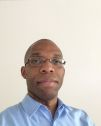
\includegraphics[width=1in,height=1.25in,clip,keepaspectratio]{Photo_Georges_Djimefo_resized.JPG}}]{Georges Parfait Djimefo Kapen}
He received a bachelor's degree in software engineering from Polytechnique Montréal in $2021$. He holds a Master's degree in Statistics from the University of Yaoundé I. He also holds another Master's degree in Mathematics from the same university.
\end{IEEEbiography}

% if you will not have a photo at all:
\begin{IEEEbiography}[{
\includegraphics[width=1in,height=1.25in,clip,keepaspectratio]{Photo_Mme_Ranwa.jpg}}]{Dr Ranwa AL MALLAH}
Dr. Ranwa Al Mallah received her Ph.D. degree in computer and software engineering from Polytechnique Montreal in $2018$.  She then joined the Security laboratory of Polytechnique Montréal as a research assistant. Shortly after, she was a Postdoctoral fellow at Toronto Metropolitan University. She was an Assistant Professor in the Department of Electrical and Computer Engineering at the Royal Military College of Canada and is now an associate professor at Polytechnique Montreal. Ms. Al Mallah has over eight years of industry experience in IT, cybersecurity and telecommunications project management. She works in the fields of artificial intelligence, adversarial machine learning, computer networks and cybersecurity.
\end{IEEEbiography}

% insert where needed to balance the two columns on the last page with
% biographies
%\newpage

\begin{IEEEbiography}[{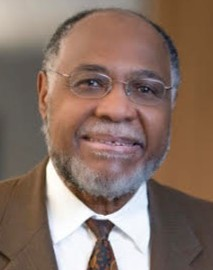
\includegraphics[width=1in,height=1.25in,clip,keepaspectratio]{samuel-pierre1.jpg}}]{Pr Samuel Pierre} SAMUEL PIERRE (Senior Member, IEEE) received the Ph.D. degree (Hons.) from Université du Quebec à Trois-Rivieres (UQTR), in May $2014$, and the Ph.D. degree (Hons.) from Université du Quebec en Outaouais (UQO), in November $2016$. He is currently a Professor with the Department of Computer and Software Engineering, Polytechnique Montréal, and the Director of the Mobile Computing and Networking Research Laboratory (LARIM). He has authored or coauthored more than $550$ technical publications, including articles in refereed archival journals, textbooks, patents, and book chapters. His research interests include wired and wireless communications, mobile computing and networking, cloud computing, and e-learning. He was a fellow of The Engineering Institute of Canada, in $2003$, and The Canadian Academy of Engineering, in $2008$. He was appointed as a member of the Order of Canada, in December $2011$. He has received several awards, including the Prix Poly $1873$ for Excellence in Teaching and Training, in $2001$ and $2005$, and the Knight of the National Order of Quebec, in $2009$. He also received the El Fasi Prize from the Agence Universitaire de la Francophonie (AUF) to highlight the action of a person who has exerted a significant influence through the quality of his expertise and the innovative nature of his achievements at the international level in the fields of research, training, development and international cooperation, governance and/or transfer of knowledge or skills, in $2017$, the Grand Prize for Professional Excellence from the Order of Engineers of Quebec (OIQ), in $2020$, and the Gold Medal from Engineers Canada, in $2021$, the promotion of Officer of the National Order of Quebec in $2022$, the JM Ham Award from IEEE Canada ($2023$) for "outstanding contributions to training the next generation of scientists and engineers in the areas of mobile computing, networking and e-learning", and the Julian C. Smith Medal of the Engineering Institute of Canada "for distinguished achievements in the development of Canada" ($2024$).
\end{IEEEbiography}

% You can push biographies down or up by placing
% a \vfill before or after them. The appropriate
% use of \vfill depends on what kind of text is
% on the last page and whether or not the columns
% are being equalized.

%\vfill

% Can be used to pull up biographies so that the bottom of the last one
% is flush with the other column.
%\enlargethispage{-5in}



% that's all folks
\end{document}


